%!TEX TS-program = xelatex
\documentclass[notes,12pt, aspectratio=169]{beamer}

\usepackage{amsmath,amsfonts,amssymb,amsthm,mathtools}  % пакеты для математики
\usepackage{minted}

\usepackage[english, russian]{babel} % выбор языка для документа
\usepackage[utf8]{inputenc} % задание utf8 кодировки исходного tex файла
\usepackage[X2,T2A]{fontenc}        % кодировка

\usepackage{fontspec}         % пакет для подгрузки шрифтов
\setmainfont{Helvetica}  % задаёт основной шрифт документа

% why do we need \newfontfamily:
% http://tex.stackexchange.com/questions/91507/
\newfontfamily{\cyrillicfonttt}{Helvetica}
\newfontfamily{\cyrillicfont}{Helvetica}
\newfontfamily{\cyrillicfontsf}{Helvetica}

\usepackage{unicode-math}     % пакет для установки математического шрифта
% \setmathfont{Neo Euler} % шрифт для математики

\usepackage{polyglossia}      % Пакет, который позволяет подгружать русские буквы
\setdefaultlanguage{russian}  % Основной язык документа
\setotherlanguage{english}    % Второстепенный язык документа

% Шрифт для кода
\setmonofont[Scale=0.85]{Monaco}
\usepackage{verbments}

\usepackage{pgfpages}
% These slides also contain speaker notes. You can print just the slides,
% just the notes, or both, depending on the setting below. Comment out the want
% you want.
%\setbeameroption{hide notes} % Only slide
%\setbeameroption{show only notes} % Only notes
%\setbeameroption{show notes on second screen=right} % Both

\usepackage{array}

\usepackage{tikz}
\usepackage{verbatim}
\setbeamertemplate{note page}{\pagecolor{yellow!5}\insertnote}
\usetikzlibrary{positioning}
\usetikzlibrary{snakes}
\usetikzlibrary{calc}
\usetikzlibrary{arrows}
\usetikzlibrary{decorations.markings}
\usetikzlibrary{shapes.misc}
\usetikzlibrary{matrix,shapes,arrows,fit,tikzmark}

\usepackage{hyperref}
\usepackage{lipsum}
\usepackage{multimedia}
\usepackage{multirow}
\usepackage{dcolumn}
\usepackage{bbm}
\newcolumntype{d}[0]{D{.}{.}{5}}

\usepackage{changepage}
\usepackage{appendixnumberbeamer}
\newcommand{\beginbackup}{
   \newcounter{framenumbervorappendix}
   \setcounter{framenumbervorappendix}{\value{framenumber}}
   \setbeamertemplate{footline}
   {
     \leavevmode%
     \hline
     box{%
       \begin{beamercolorbox}[wd=\paperwidth,ht=2.25ex,dp=1ex,right]{footlinecolor}%
%         \insertframenumber  \hspace*{2ex} 
       \end{beamercolorbox}}%
     \vskip0pt%
   }
 }
\newcommand{\backupend}{
   \addtocounter{framenumbervorappendix}{-\value{framenumber}}
   \addtocounter{framenumber}{\value{framenumbervorappendix}} 
}

% для имитации питоновского синтаксиса 
\newcommand{\pgr}[1]{{\color{green} \textbf{#1}}}


%%%%%%%%%% Работа с картинками %%%%%%%%%
\usepackage{graphicx}                  % Для вставки рисунков
\usepackage{graphics}
\graphicspath{{images/},{imagess/}}    % можно указать папки с картинками
\usepackage{wrapfig}                   % Обтекание рисунков и таблиц текстом

\usepackage[space]{grffile}
\usepackage{booktabs}

% These are my colors -- there are many like them, but these ones are mine.
\definecolor{blue}{RGB}{0,114,178}
\definecolor{red}{RGB}{213,94,0}
\definecolor{yellow}{RGB}{240,228,66}
\definecolor{green}{RGB}{0,128, 0}

\hypersetup{
  colorlinks=false,
  linkbordercolor = {white},
  linkcolor = {blue}
}


%% I use a beige off white for my background
\definecolor{MyBackground}{RGB}{255,253,218}

%% Uncomment this if you want to change the background color to something else
%\setbeamercolor{background canvas}{bg=MyBackground}

%% Change the bg color to adjust your transition slide background color!
\newenvironment{transitionframe}{
  \setbeamercolor{background canvas}{bg=yellow}
  \begin{frame}}{
    \end{frame}
}

\setbeamercolor{frametitle}{fg=blue}
\setbeamercolor{title}{fg=black}
\setbeamertemplate{footline}[frame number]
\setbeamertemplate{navigation symbols}{} 
\setbeamertemplate{itemize items}{-}
\setbeamercolor{itemize item}{fg=blue}
\setbeamercolor{itemize subitem}{fg=blue}
\setbeamercolor{enumerate item}{fg=blue}
\setbeamercolor{enumerate subitem}{fg=blue}
\setbeamercolor{button}{bg=MyBackground,fg=blue,}


% If you like road maps, rather than having clutter at the top, have a roadmap show up at the end of each section 
% (and after your introduction)
% Uncomment this is if you want the roadmap!
% \AtBeginSection[]
% {
%    \begin{frame}
%        \frametitle{Roadmap of Talk}
%        \tableofcontents[currentsection]
%    \end{frame}
% }
\setbeamercolor{section in toc}{fg=blue}
\setbeamercolor{subsection in toc}{fg=red}
\setbeamersize{text margin left=1em,text margin right=1em} 

% списки, которые растягиваются на всю величину слайда 
\newenvironment{wideitemize}{\itemize\addtolength{\itemsep}{10pt}}{\enditemize}


\title[]{\textcolor{blue}{Глубокое обучение и вообще}}
\author{Ульянкин Филипп и Соловей Влад}
\date{\today}

\begin{document}

%%% TIKZ STUFF
\tikzset{   
        every picture/.style={remember picture,baseline},
        every node/.style={anchor=base,align=center,outer sep=1.5pt},
        every path/.style={thick},
        }
\newcommand\marktopleft[1]{%
    \tikz[overlay,remember picture] 
        \node (marker-#1-a) at (-.3em,.3em) {};%
}
\newcommand\markbottomright[2]{%
    \tikz[overlay,remember picture] 
        \node (marker-#1-b) at (0em,0em) {};%
}
\tikzstyle{every picture}+=[remember picture] 
\tikzstyle{mybox} =[draw=black, very thick, rectangle, inner sep=10pt, inner ysep=20pt]
\tikzstyle{fancytitle} =[draw=black,fill=red, text=white]
%%%% END TIKZ STUFF

\begin{frame}
\maketitle
\centering \textbf{\color{blue} Посиделка 7:}  Что видет сетки, локализация, сегментация, перенос стиля
\end{frame}

\begin{frame}{Agenda} 
\begin{wideitemize}
	\item Что видят свёрточные сетки? 
	\item Перенос стиля
	\item Локализация и сегментация
\end{wideitemize}
\end{frame}



 \begin{transitionframe}
	\begin{center}
		\Huge  Что видят нейросетки
	\end{center}
\end{transitionframe}





\begin{transitionframe}
	\begin{center}
		\Huge Перенос стиля 
	\end{center}
\end{transitionframe}


\begin{frame}{Приложение Prisma}
\begin{center}
	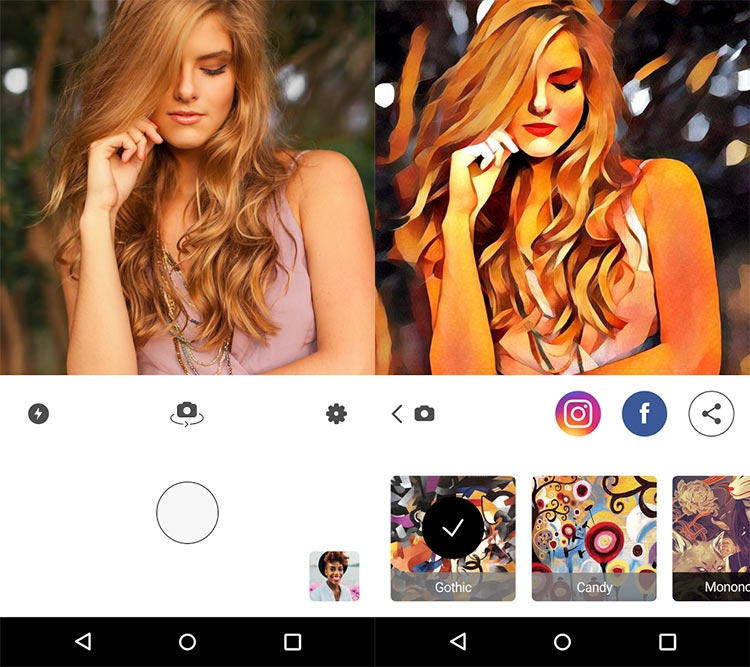
\includegraphics[width=.5\linewidth]{prisma.jpg}
\end{center}
\end{frame}


\begin{frame}{Перенос стиля}
\begin{center}
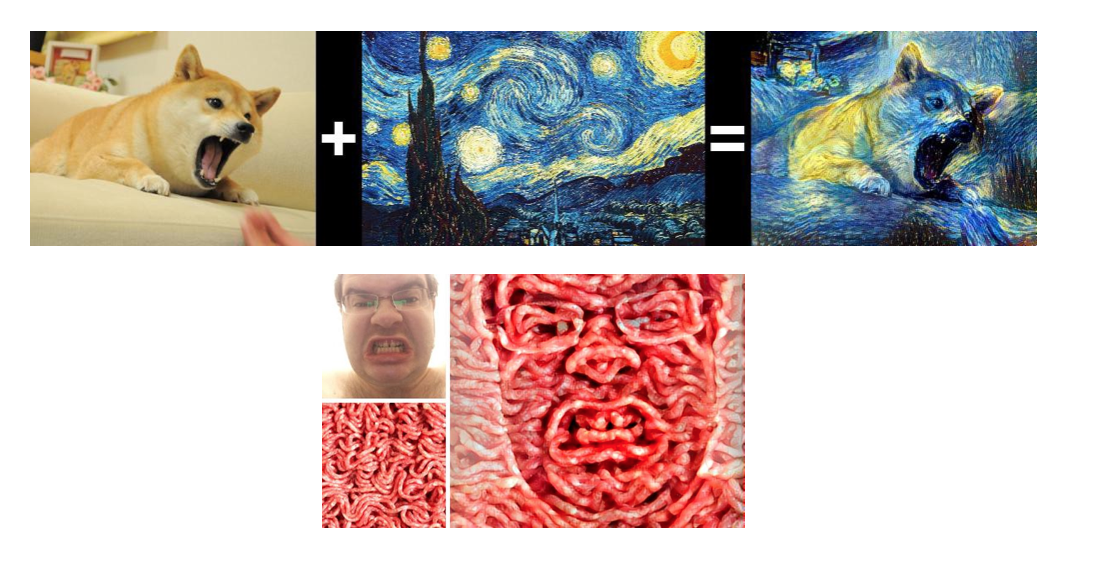
\includegraphics[width=.95\linewidth]{transfer_style.png}
\end{center}
\end{frame}


\begin{frame}{Перенос стиля}
\begin{center}
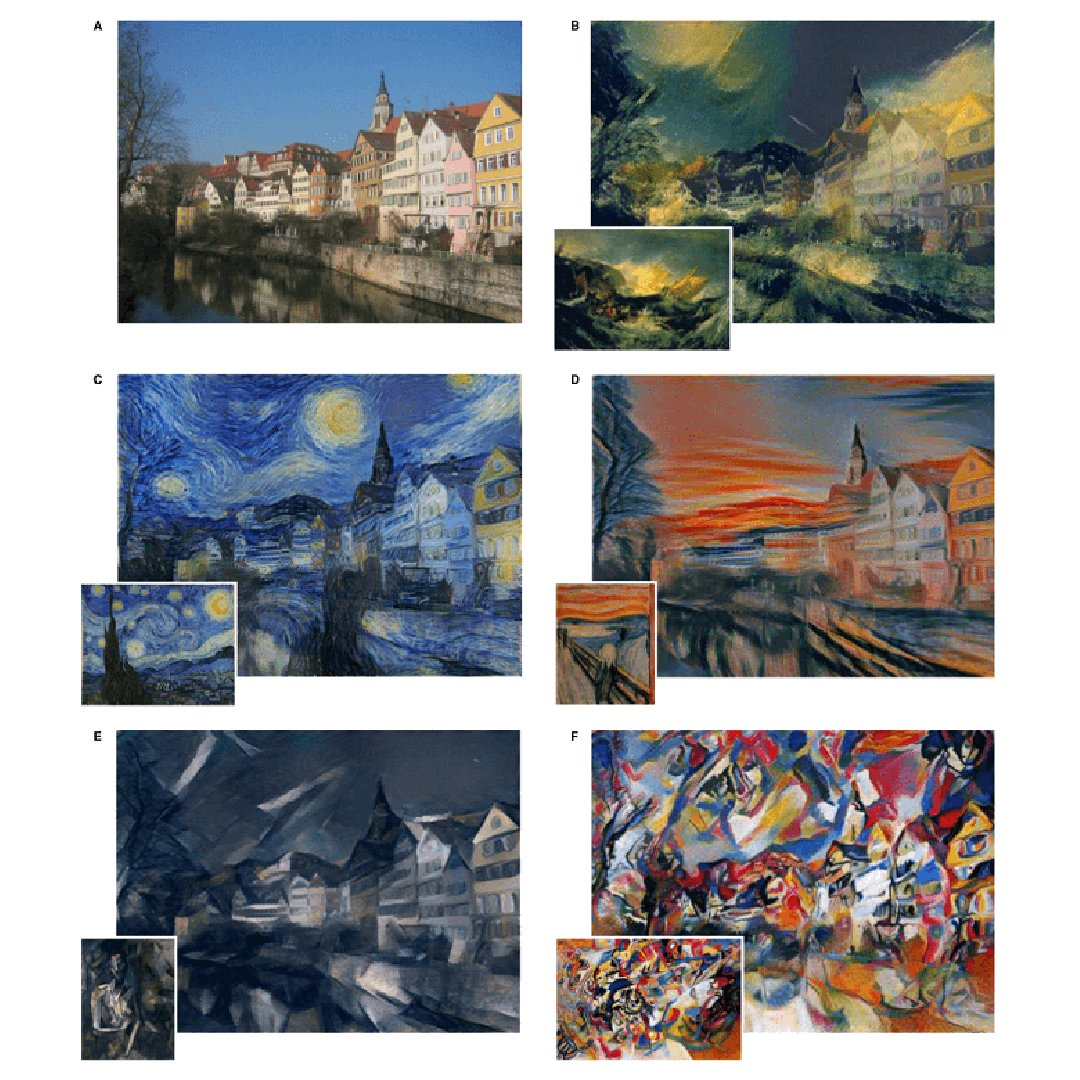
\includegraphics[width=.5\linewidth]{transfer_style_2.jpg}
\end{center}
\end{frame}


\begin{frame}
\begin{center}
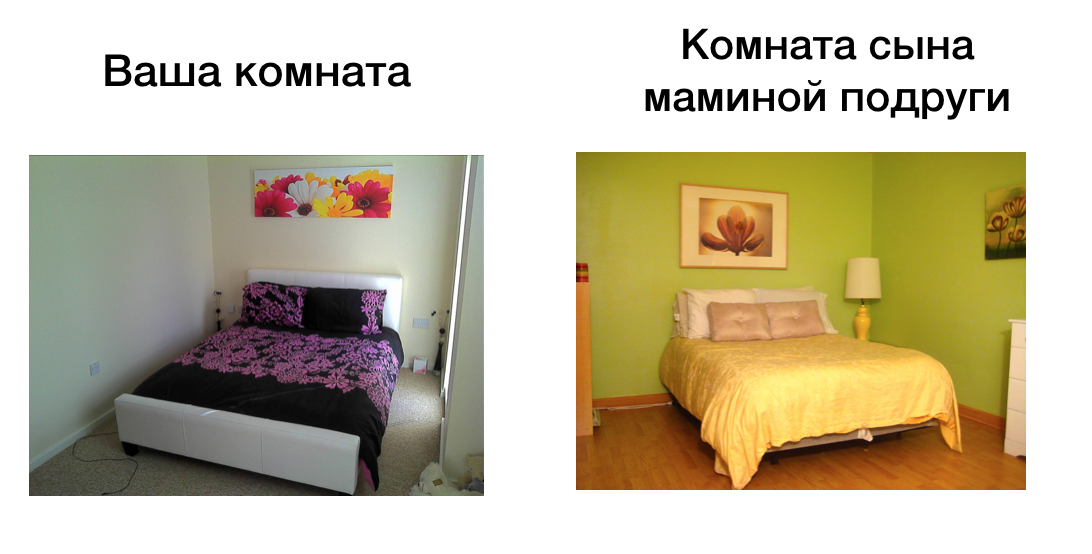
\includegraphics[width=.9\linewidth]{mom_room_1.png}
\end{center}

\vfill
\footnotesize
{\color{blue} \url{https://habr.com/ru/post/402665/}} \newline 
{\color{blue} \url{https://github.com/LouieYang/deep-photo-styletransfer-tf}} 
\end{frame}


\begin{frame}
\begin{center}
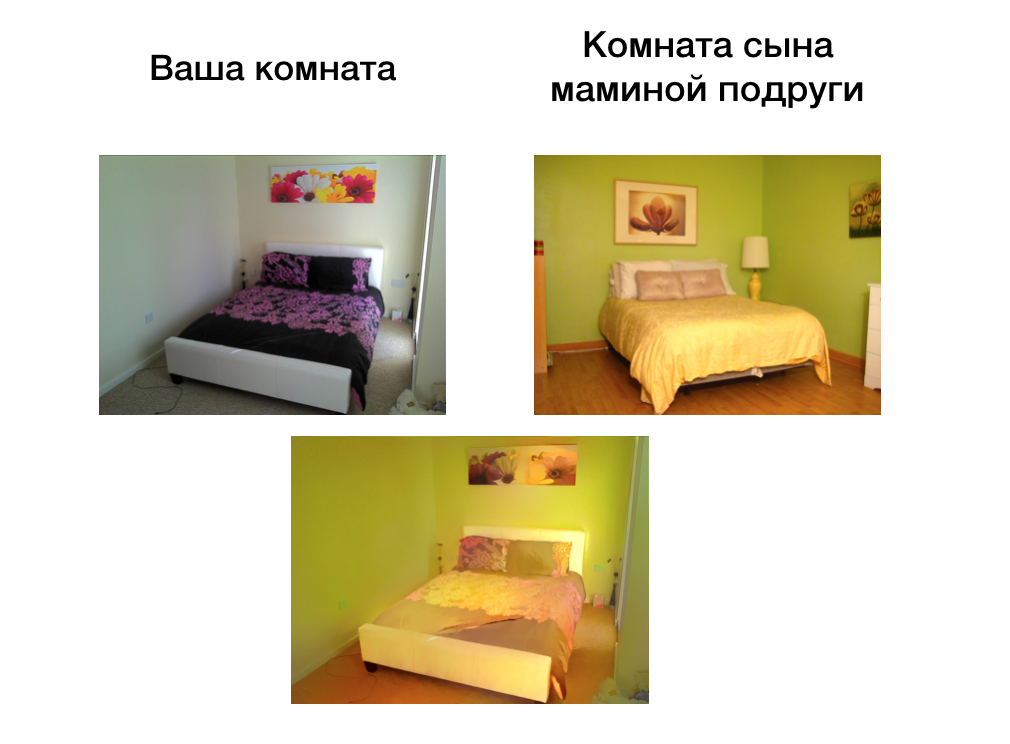
\includegraphics[width=.78\linewidth]{mom_room_2.png}
\end{center}
\end{frame}


\begin{frame}
\begin{center}
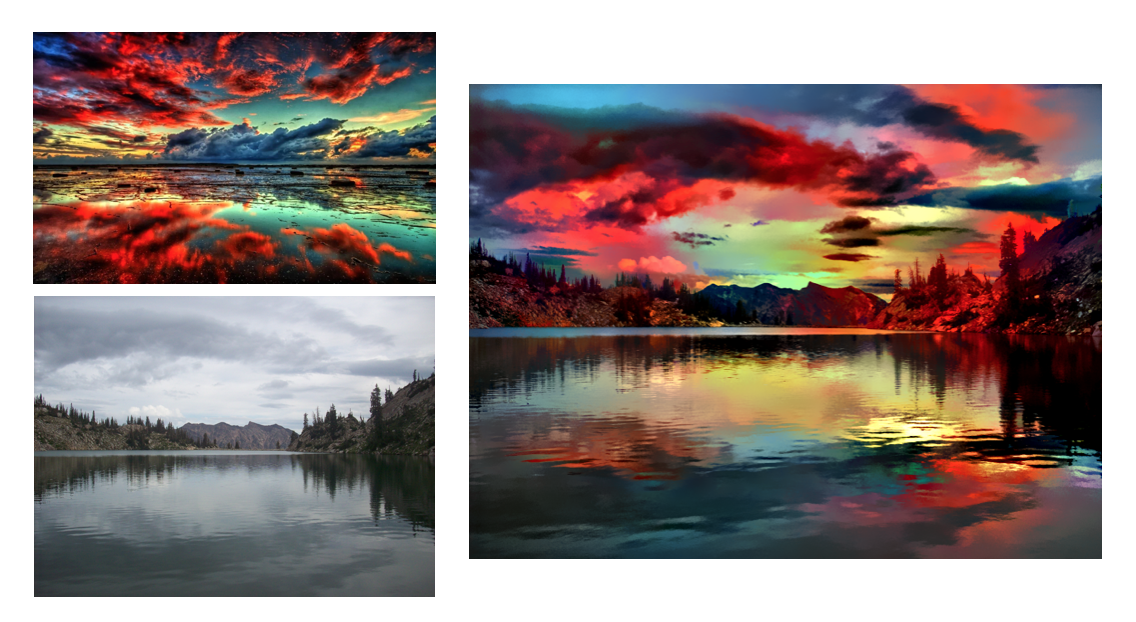
\includegraphics[width=.9\linewidth]{mom_room_3.png}
\end{center}
\end{frame}


\begin{frame}
\begin{center}
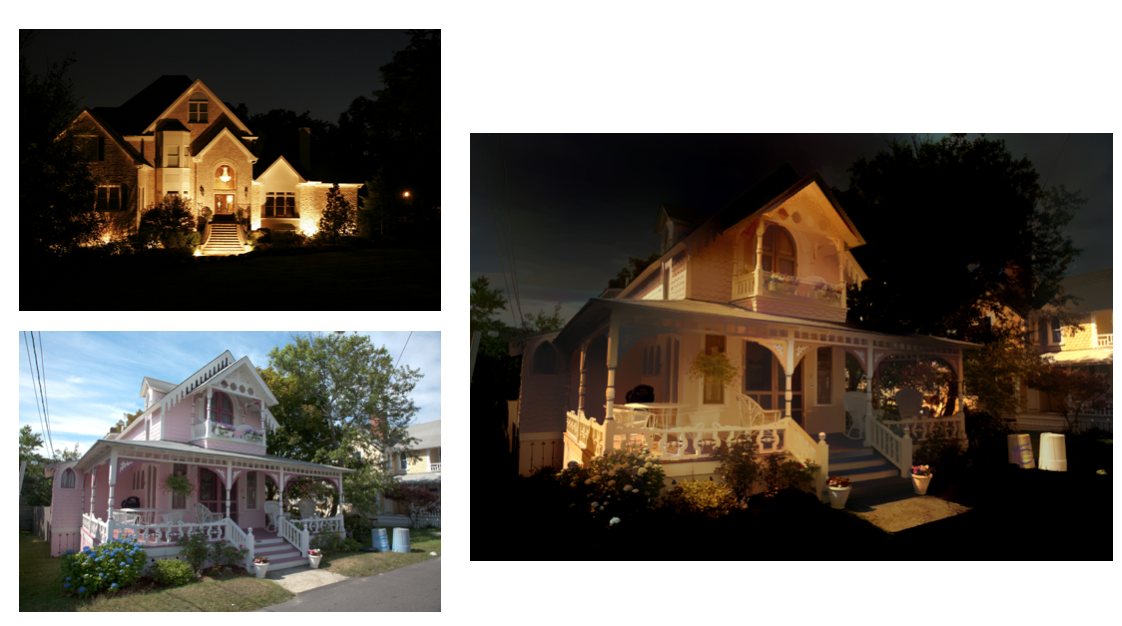
\includegraphics[width=.9\linewidth]{mom_room_4.png}
\end{center}
\end{frame}


\begin{frame}{Опять этот слайд!}
\begin{center}
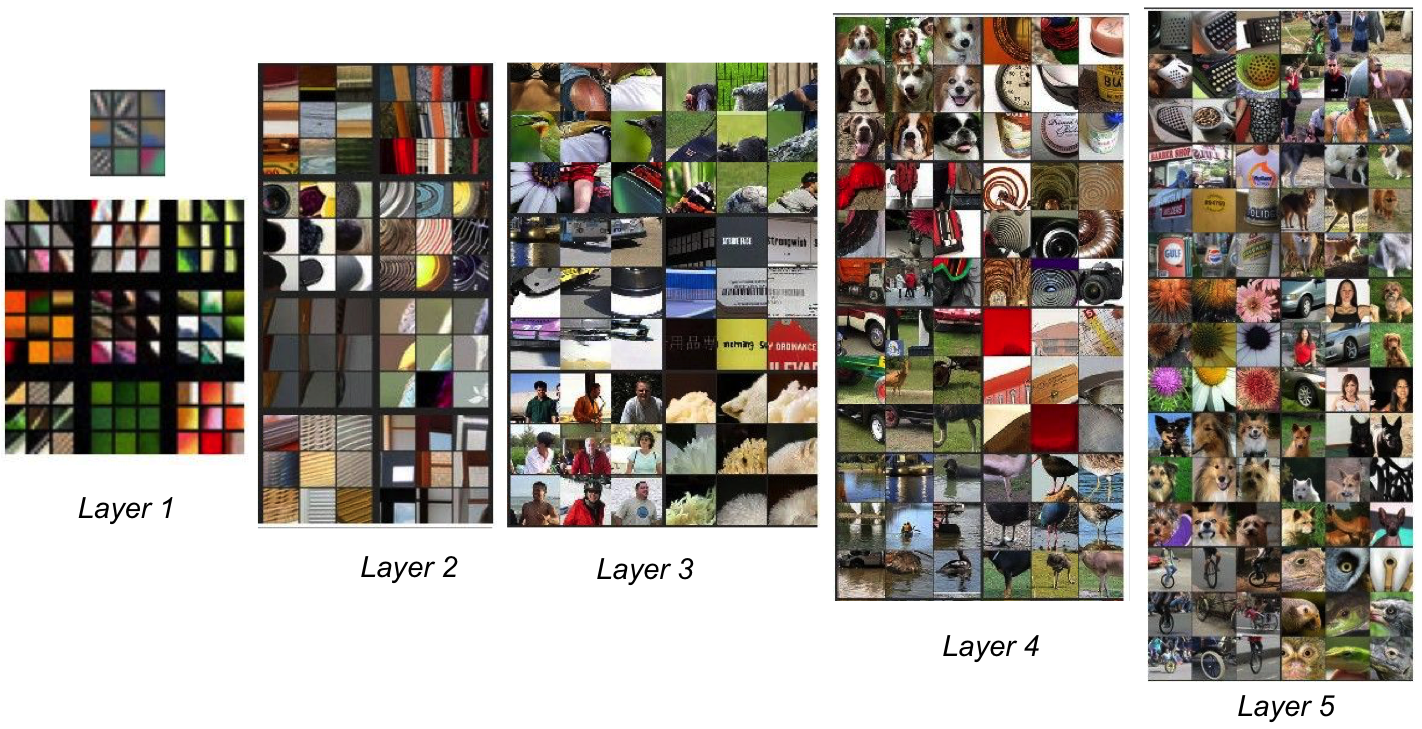
\includegraphics[width=.9\linewidth]{cnn_vis.png}
\end{center}

Есть несколько способов заглянуть внутрь свёрточной сетки, мы сейчас посмотрим на один из них
\end{frame}

\begin{frame}
\begin{center}
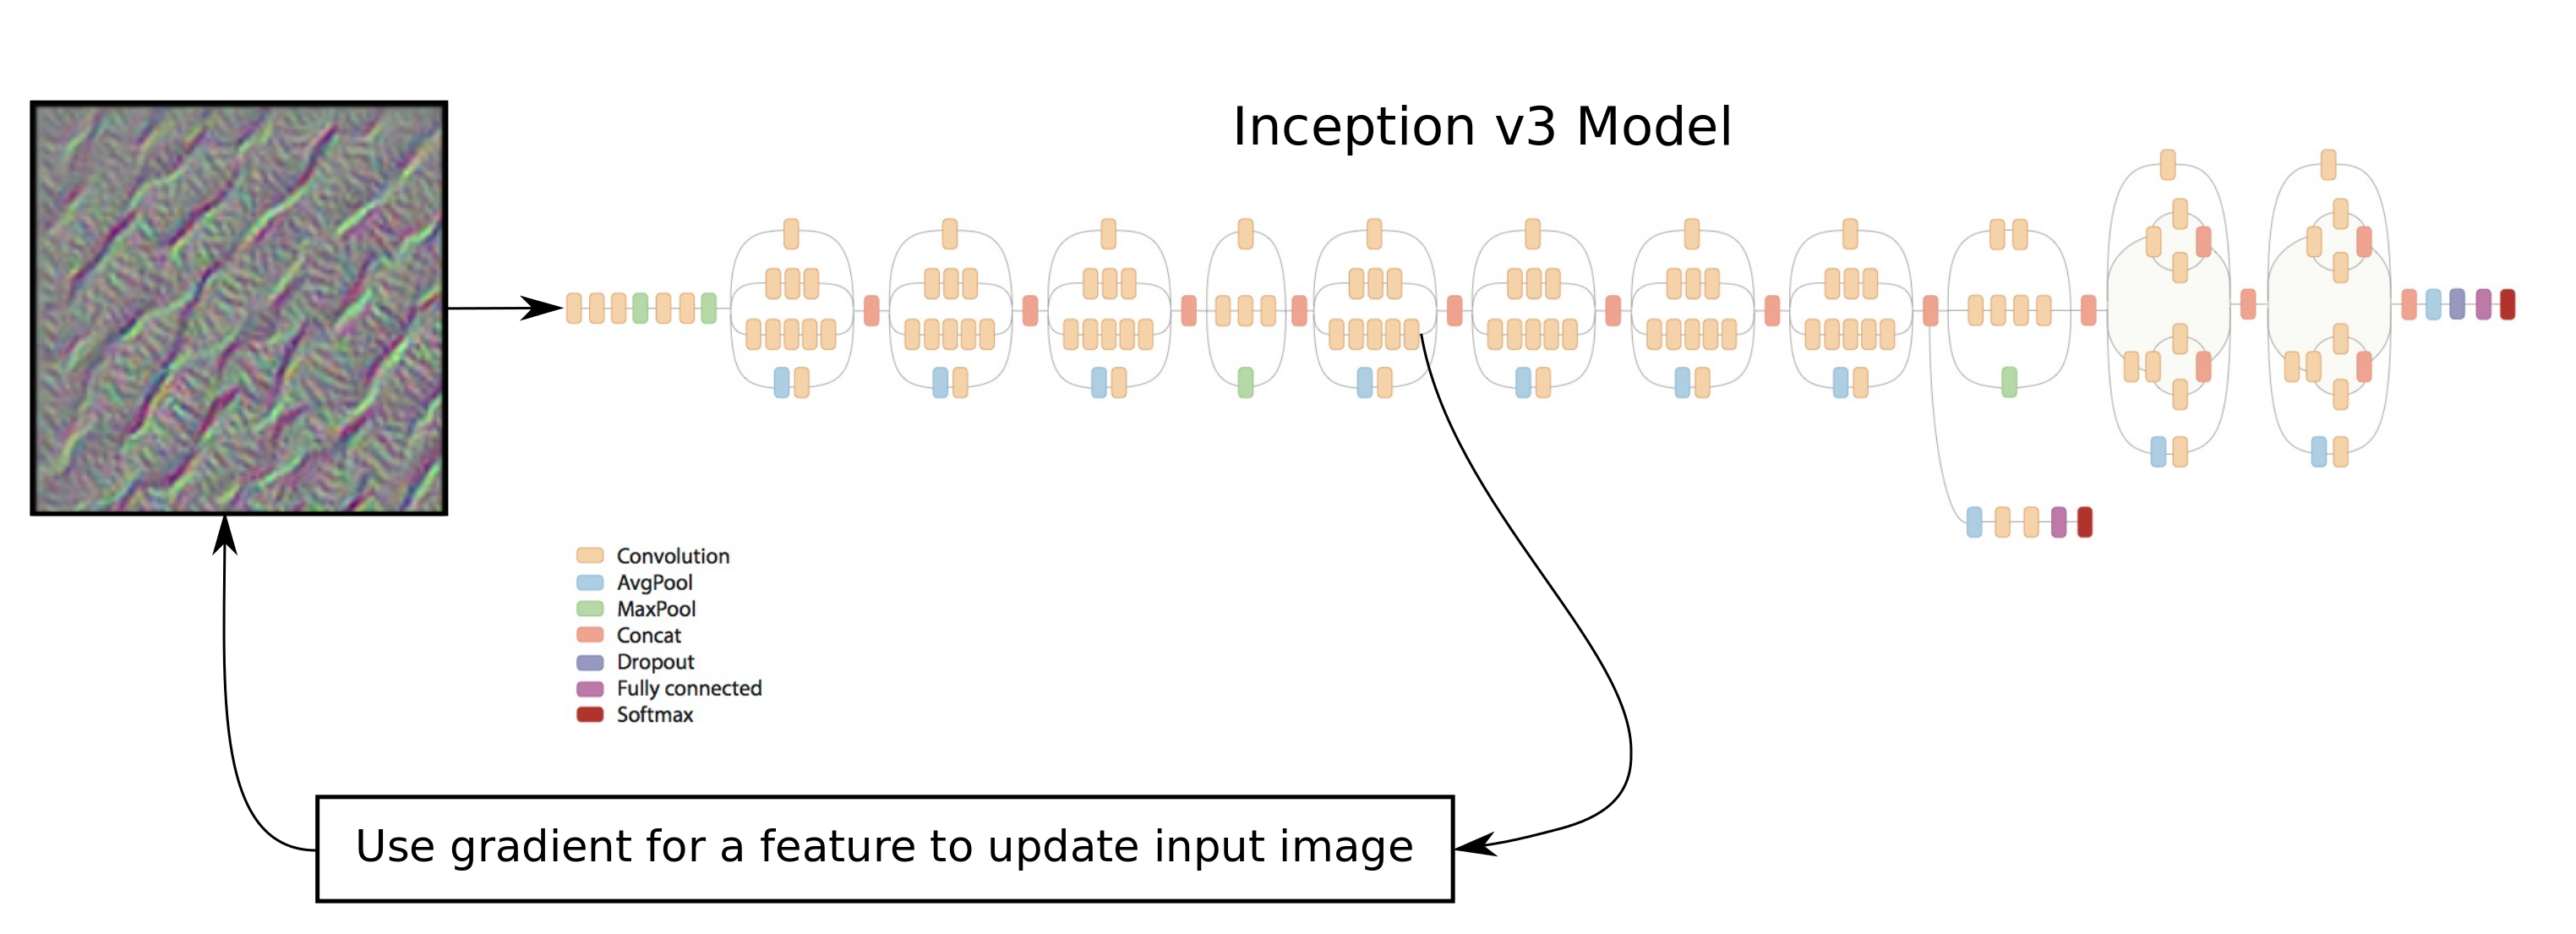
\includegraphics[width=.95\linewidth]{how_nn_see.png}
\end{center}
\end{frame}


\begin{frame}{Пример из вашей домашки}
\begin{center}
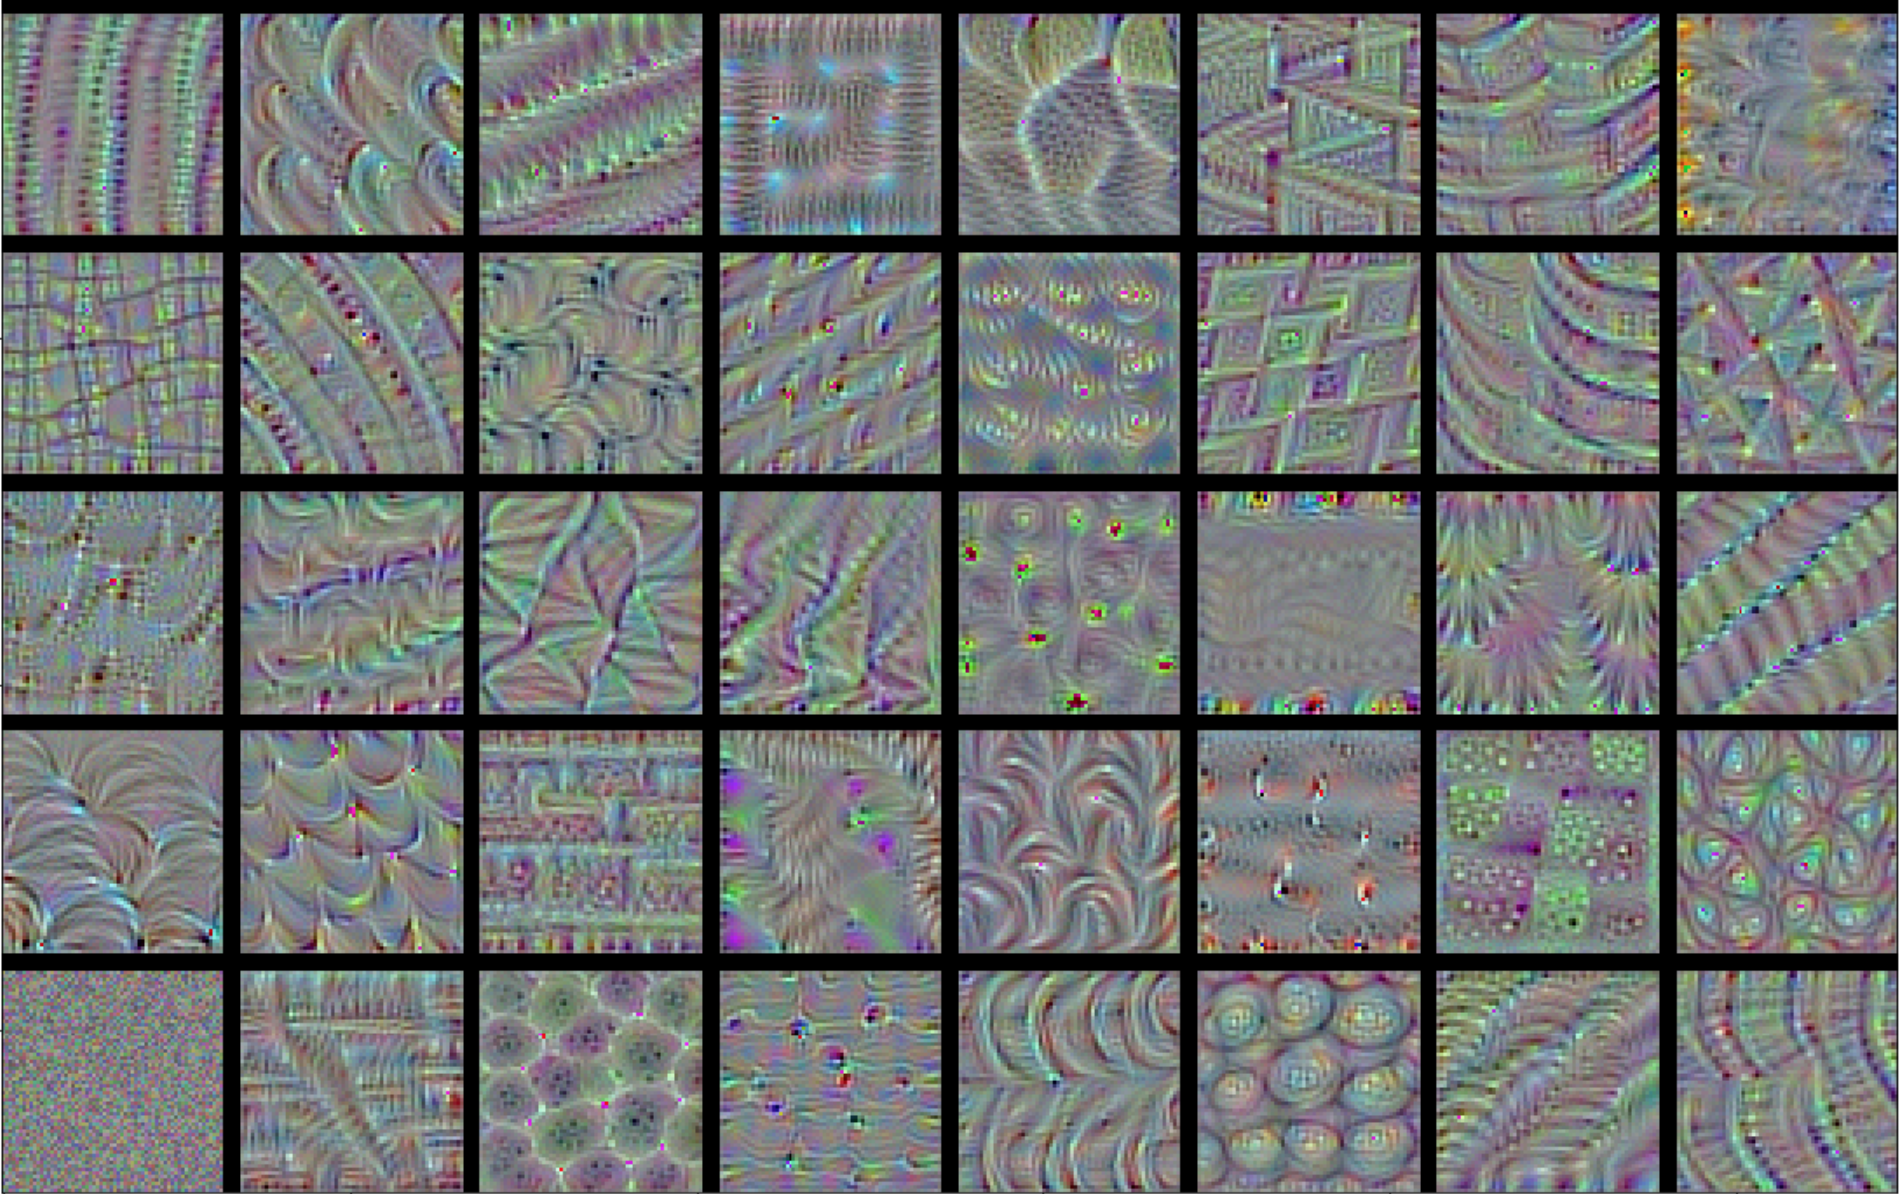
\includegraphics[width=.8\linewidth]{hw_example.png}
\end{center}
\end{frame}

\begin{frame}{Что видит свёртка}
\begin{wideitemize}

\item На вход идет пустое изображение, мы хотим изменить его пиксели так, чтобы активация конкретной свёртки была максимальной 

\item Максимизируем среднее значение свёртки по пикселям 

\item Шаг градиентного спуска: меняем пиксили так, чтобы свёртка выдавала на выход более большие значение 

\item На входной карточке постепенно прорисовывается шаблон, который возбуждает соотвествующую свёртку

\item Если на вход в сетку подсунуть не пустую карточку, а какое-то изображение, то фильтр отрисуется на нём. Если эту процедуру немного подправить, получится наркомания под названием \alert{Deep dream}
\end{wideitemize}
\end{frame}

\begin{frame}{Deep dream}
\begin{center}
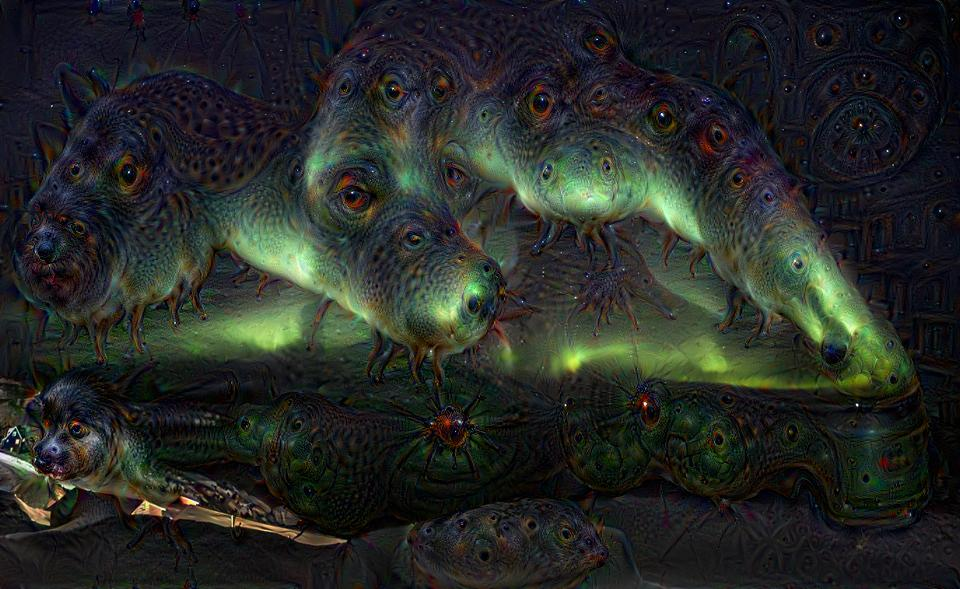
\includegraphics[width=.7\linewidth]{wtf1.jpg}
\end{center}
\vfill
\footnotesize
{\color{blue} \url{https://nplus1.ru/material/2015/07/13/use}}
\end{frame}


\begin{frame}{Content loss}
\begin{center}
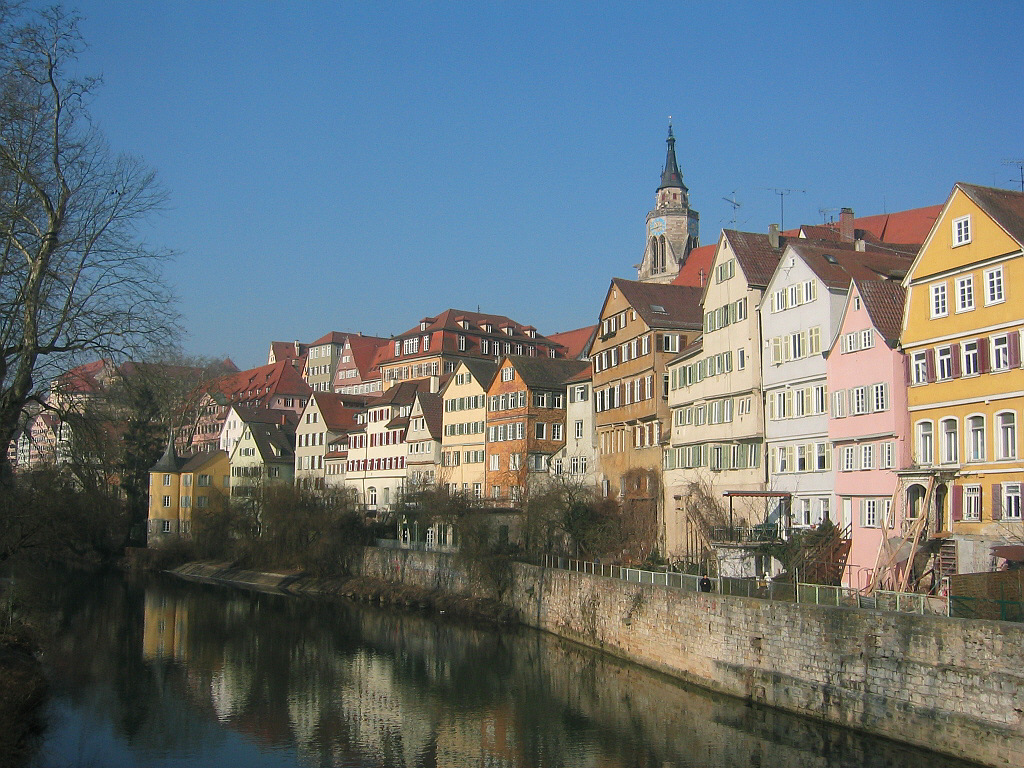
\includegraphics[width=.6\linewidth]{content_image.jpg}
\end{center}
\vfill
\footnotesize
{\color{blue} \url{https://habr.com/ru/company/mailru/blog/306916/}}
\end{frame}

\begin{frame}{Content loss}
\begin{center}
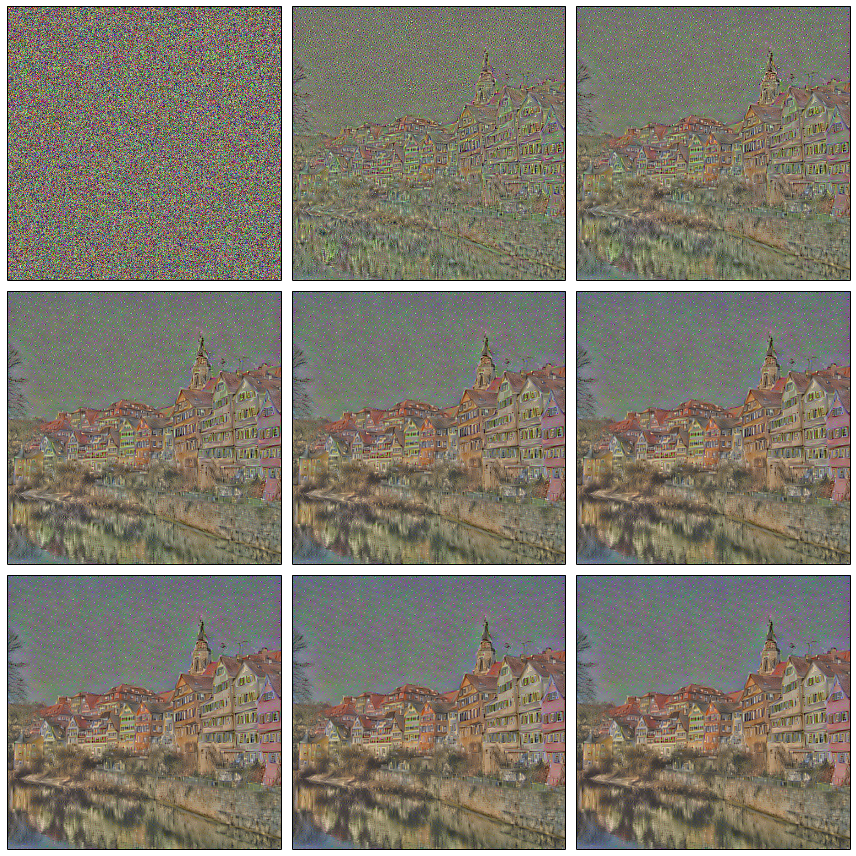
\includegraphics[width=.5\linewidth]{content1.png}
\end{center}
\vfill
\footnotesize
{\color{blue} \url{https://habr.com/ru/company/mailru/blog/306916/}}
\end{frame}



\begin{frame}{Style loss}
\begin{center}
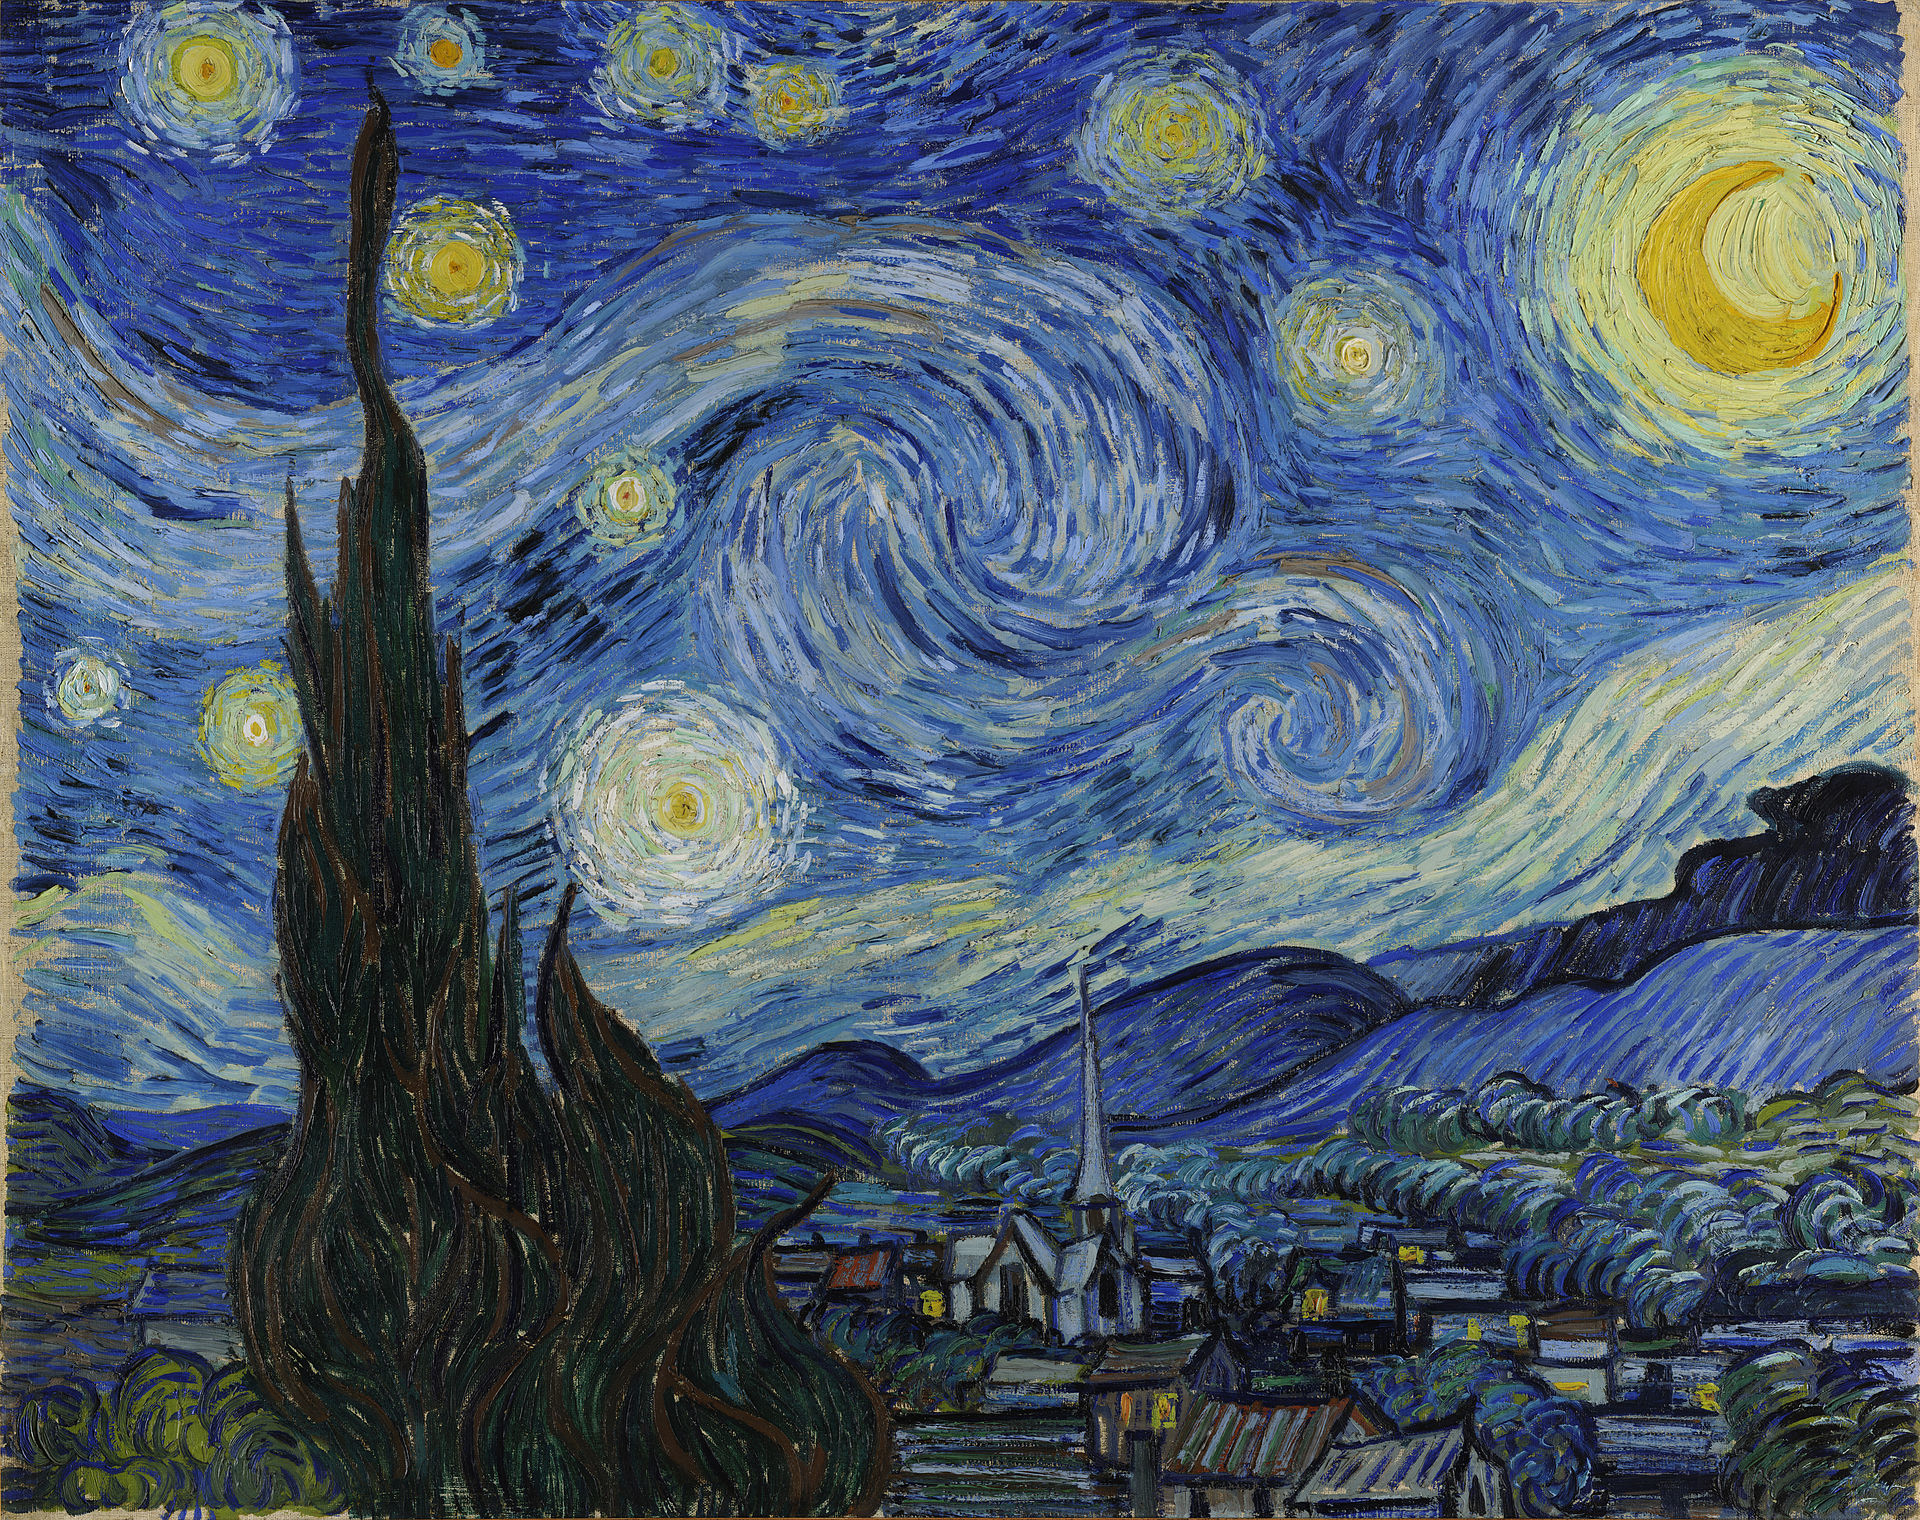
\includegraphics[width=.6\linewidth]{style_image.jpg}
\end{center}
\vfill
\footnotesize
{\color{blue} \url{https://habr.com/ru/company/mailru/blog/306916/}}
\end{frame}

\begin{frame}{Style loss}
\begin{center}
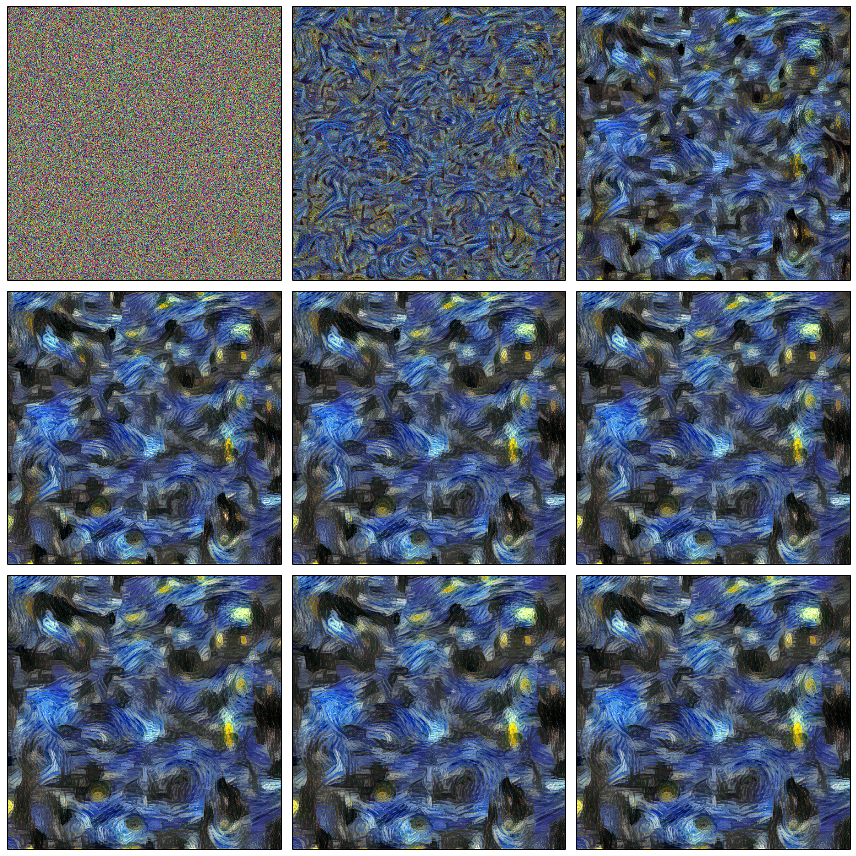
\includegraphics[width=.5\linewidth]{style1.png}
\end{center}
\vfill
\footnotesize
{\color{blue} \url{https://habr.com/ru/company/mailru/blog/306916/}}
\end{frame}


\begin{frame}{Смесь нескольких стилей}
\begin{center}
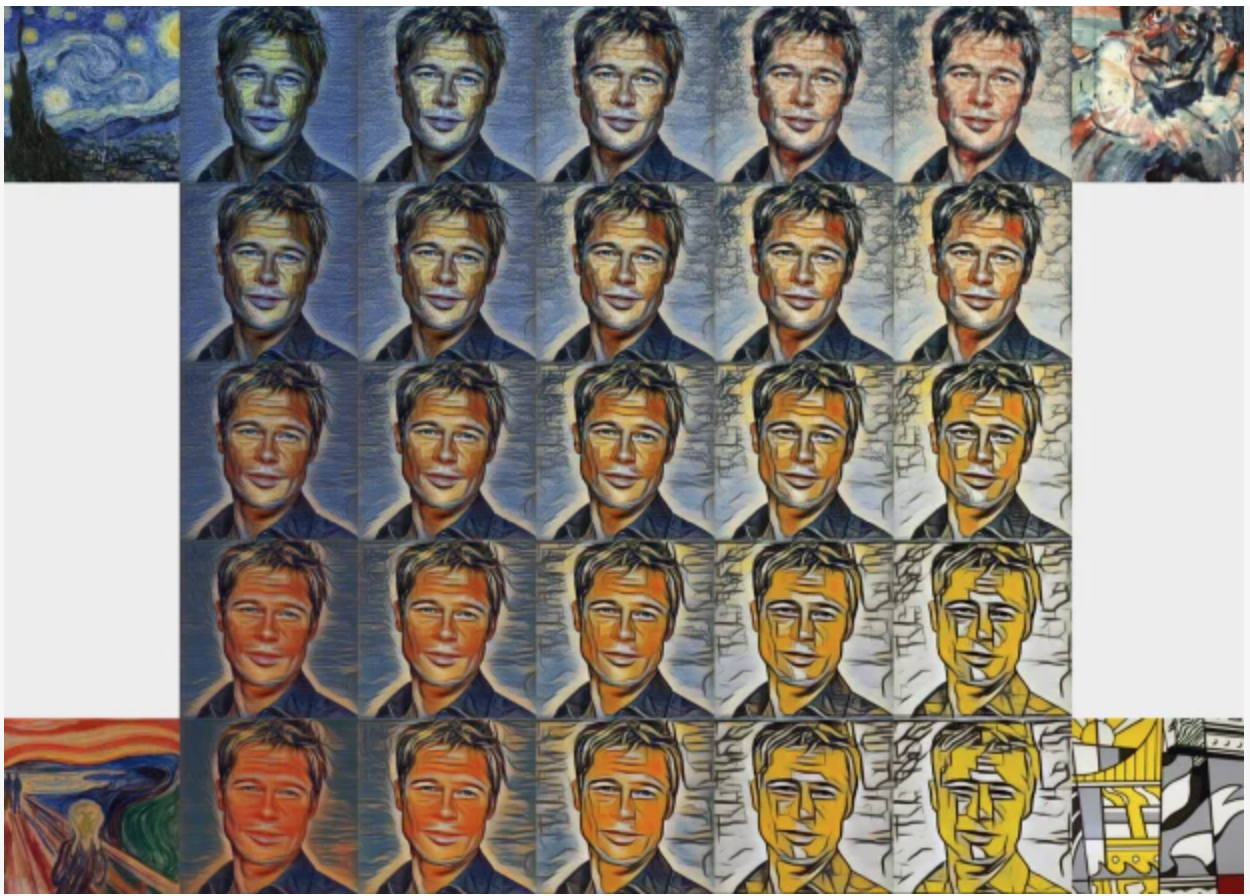
\includegraphics[width=.6\linewidth]{brad.png}
\end{center}
\vfill
\footnotesize
{\color{blue} \url{https://arxiv.org/pdf/1610.07629.pdf}} \ 
\end{frame}

\begin{transitionframe}
\begin{center}
\Huge Переносим стиль!
\end{center}
\end{transitionframe}





 \begin{transitionframe}
	\begin{center}
		\Huge  Сегментация и локализация изображений
	\end{center}
\end{transitionframe}


\begin{frame}{Сегментация и локализация}
\begin{center}
	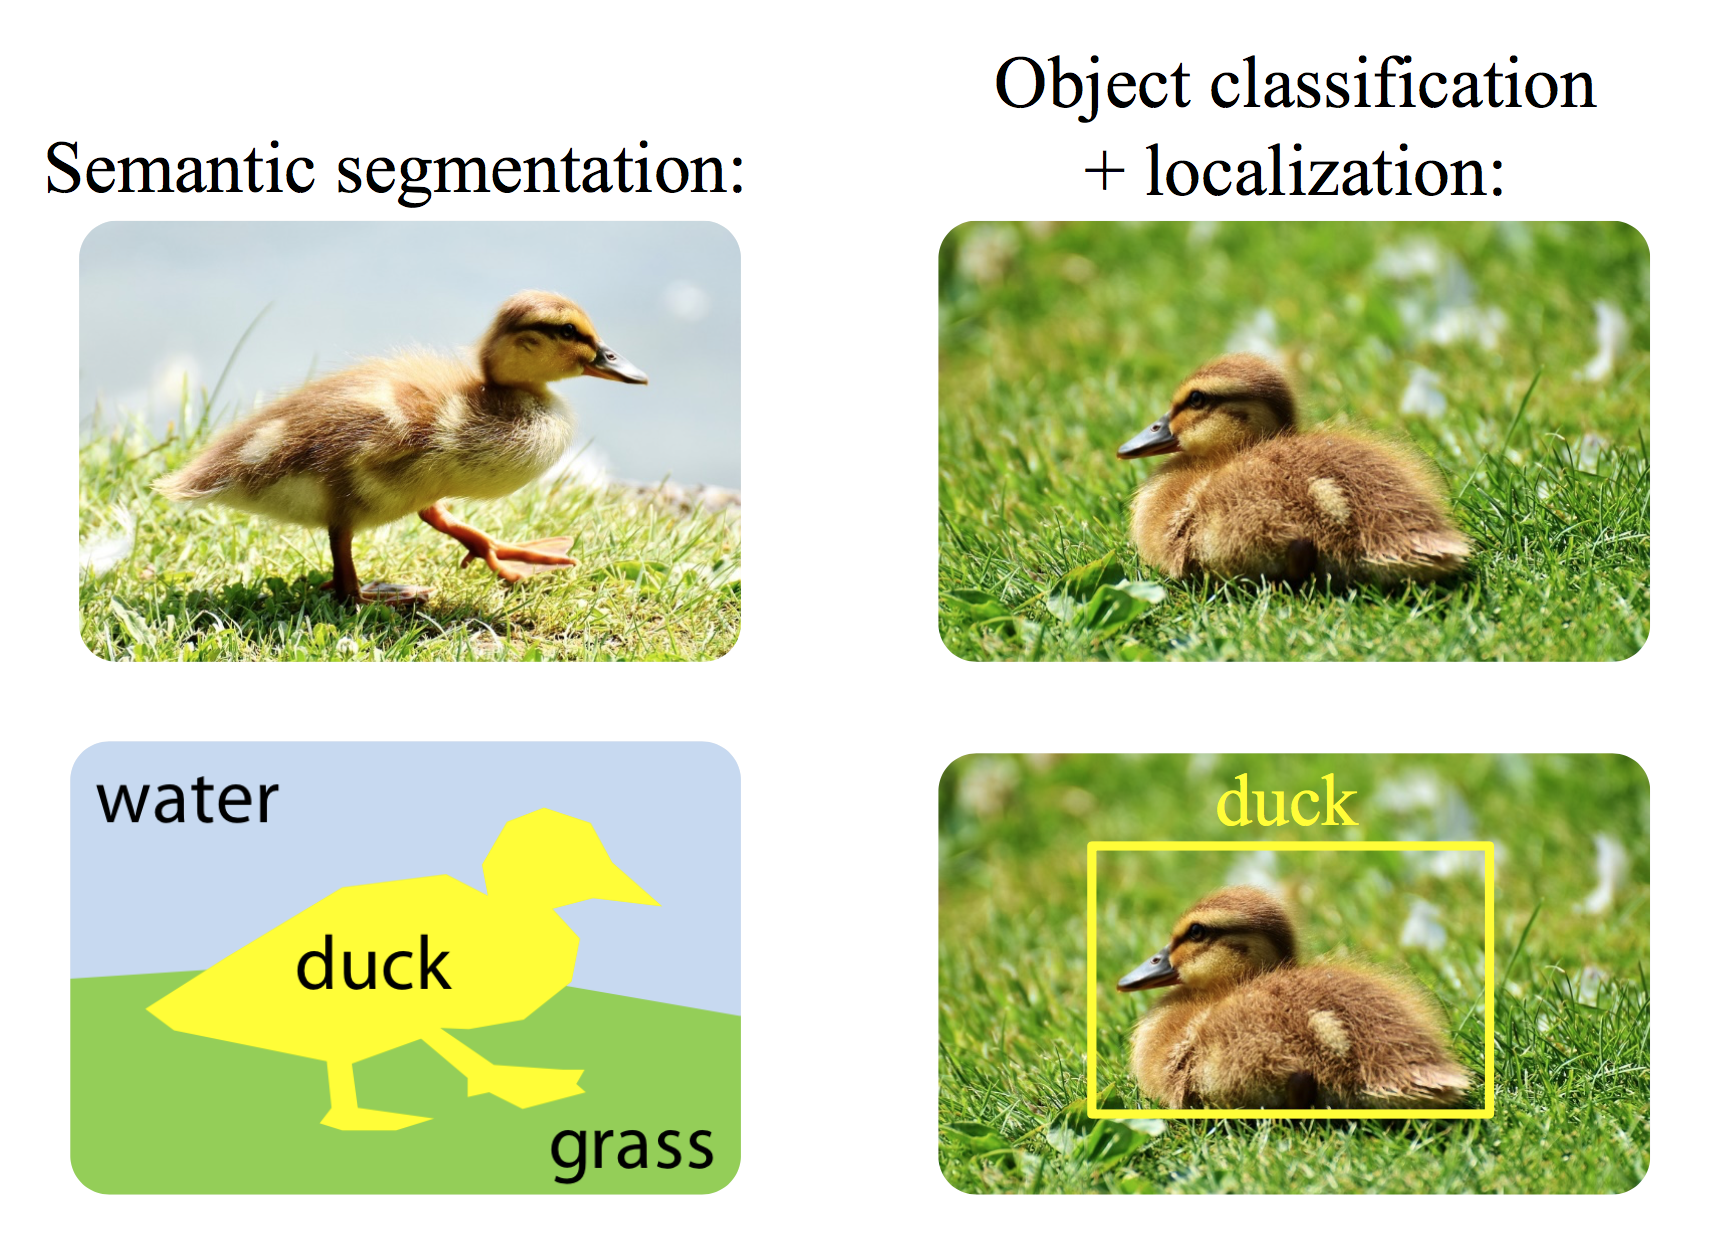
\includegraphics[width=.7\linewidth]{duck.png}
\end{center}
\end{frame}


\begin{frame}{Примеры}
\begin{center}
	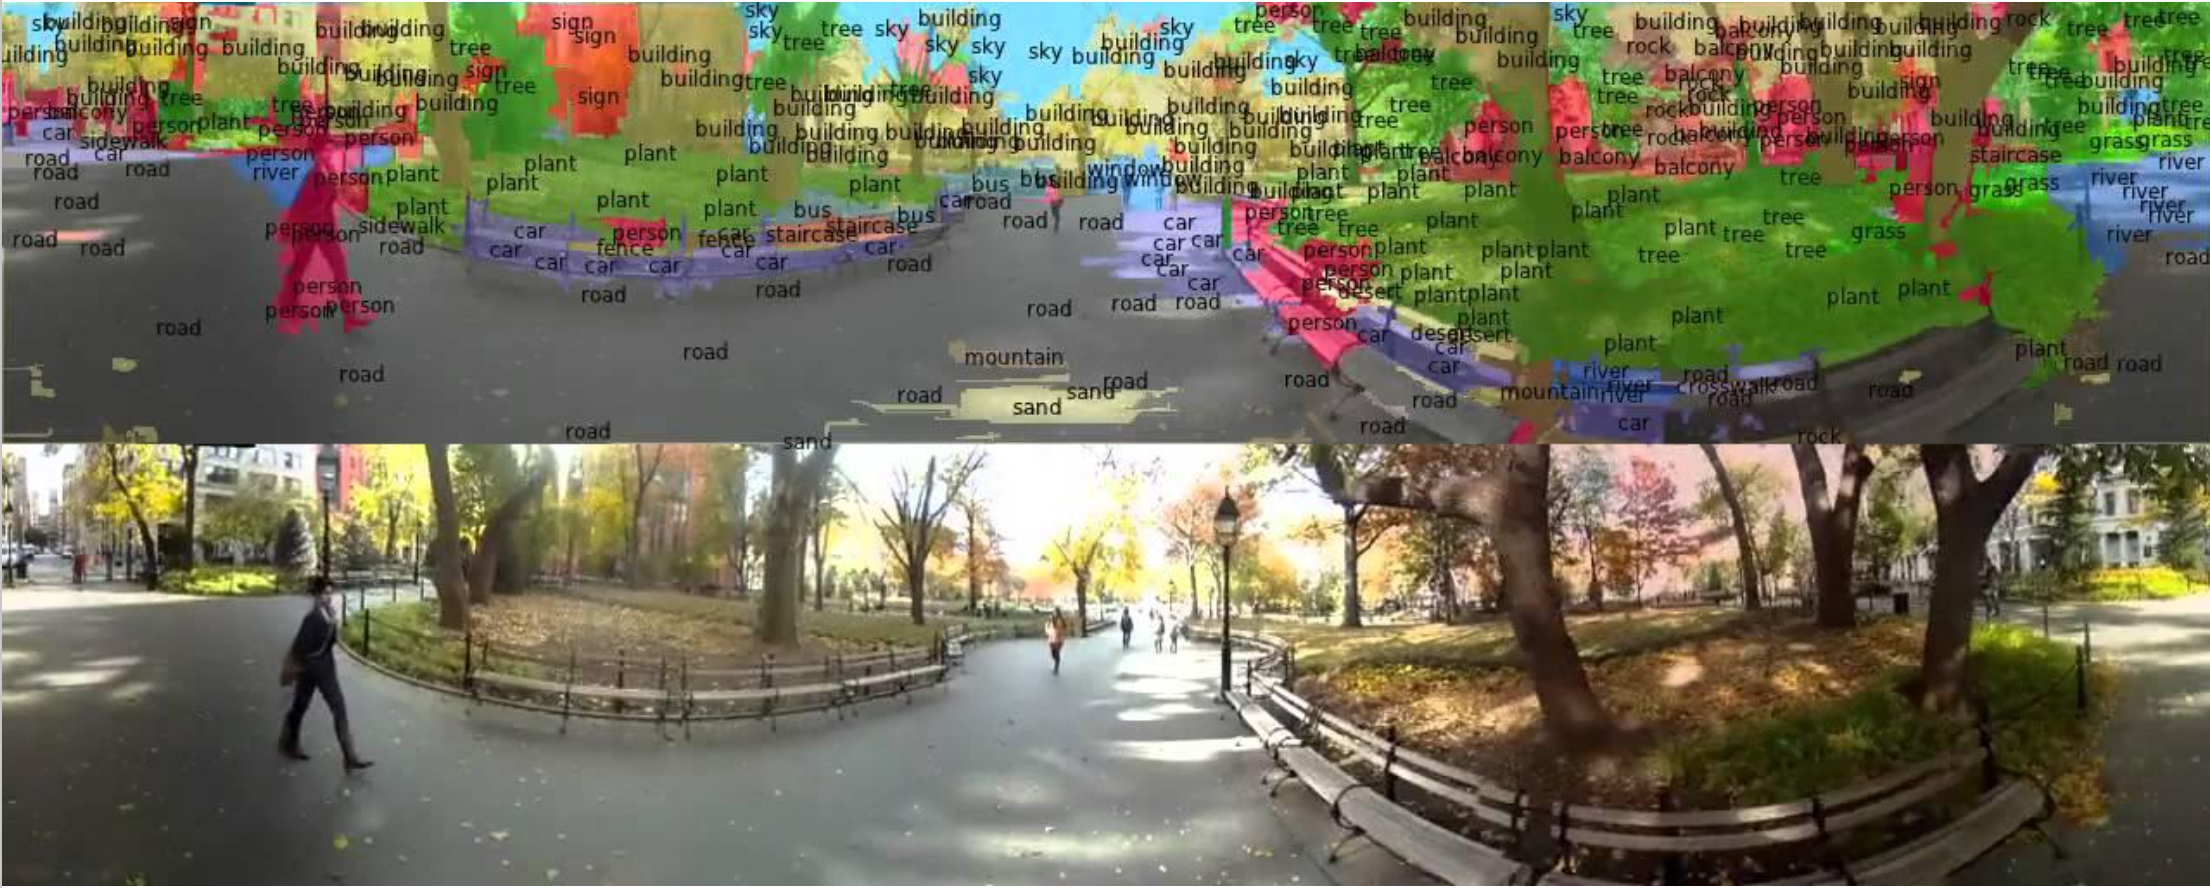
\includegraphics[width=.9\linewidth]{seg.png}
\end{center}

\vfill
\footnotesize
{\color{blue} \url{https://www.youtube.com/watch?v=ZJMtDRbqH40}}
\end{frame}


\begin{frame}{Сегментация}
\begin{center}
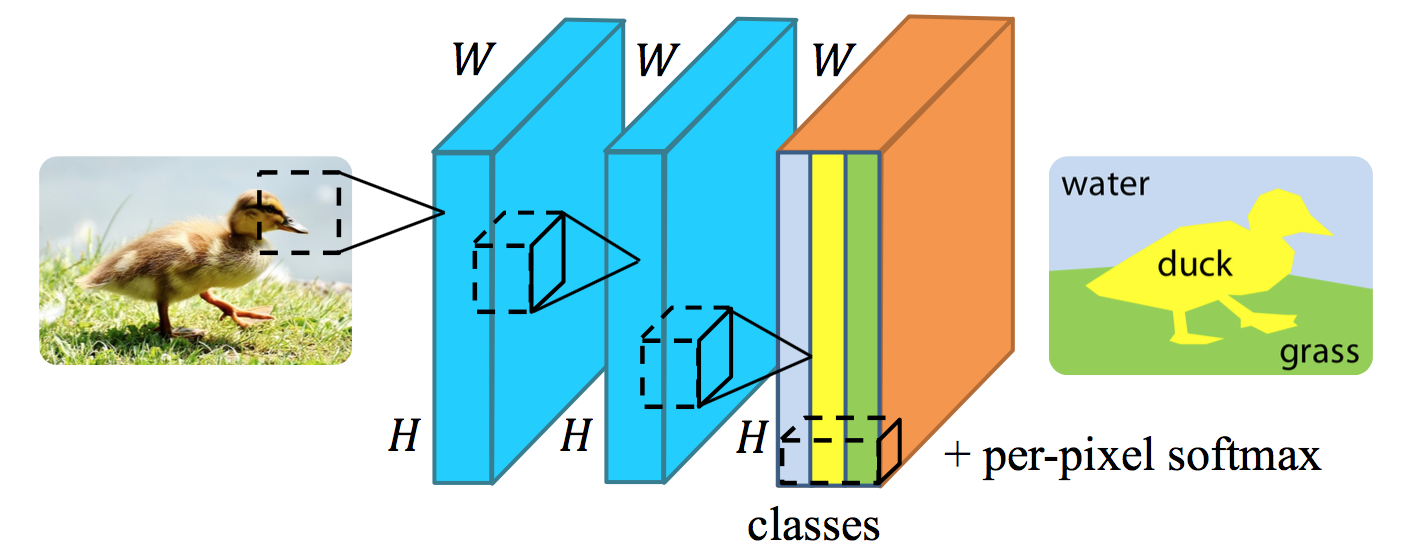
\includegraphics[width=.9\linewidth]{duck_1.png}
\end{center}
\begin{wideitemize}
\item Нам нужно научиться классифицировать каждый пиксель
\item Куча свёрток и попиксельный softmax без пулинга (наивный подход)
\end{wideitemize}
\end{frame}


\begin{frame}{Сегментация}
\begin{center}
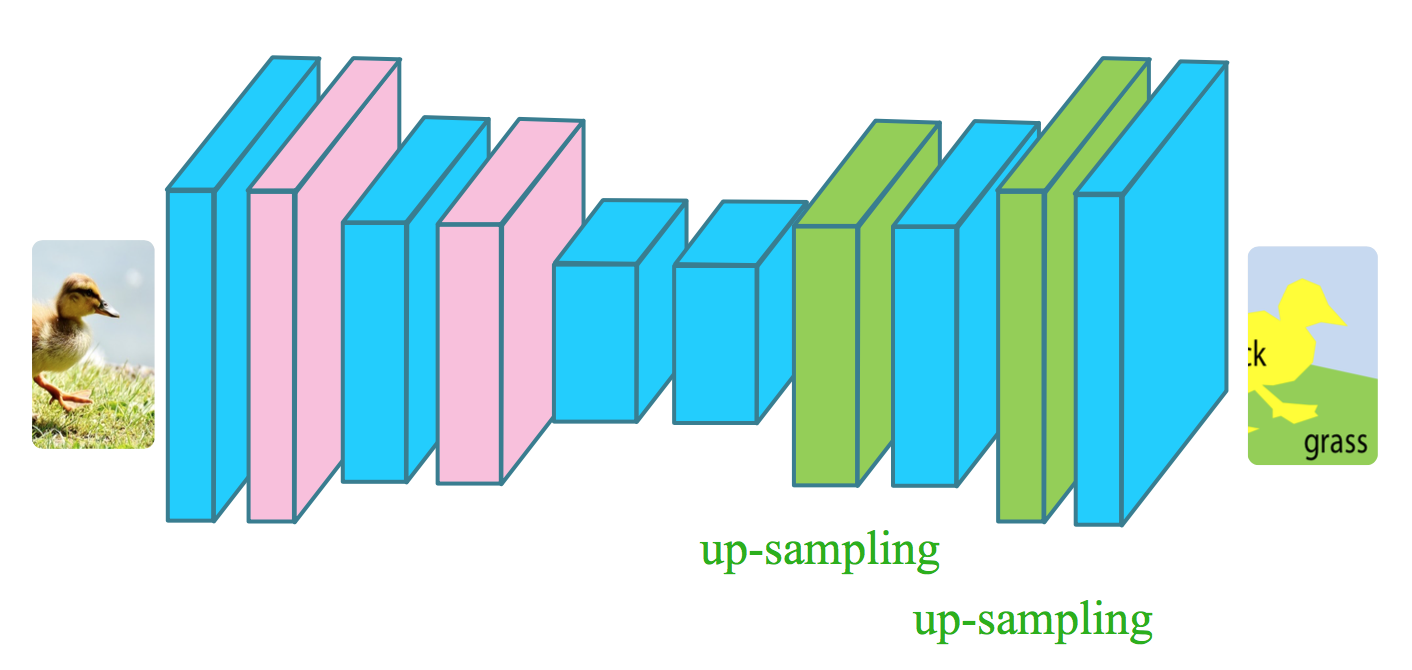
\includegraphics[width=.8\linewidth]{duck_2.png}
\end{center}
\begin{itemize}
\item Если захотим добавить пулинг, придётся делать анпулинг
\end{itemize}
\end{frame}


\begin{frame}{Nearest neighbor unpooling}
\begin{center}
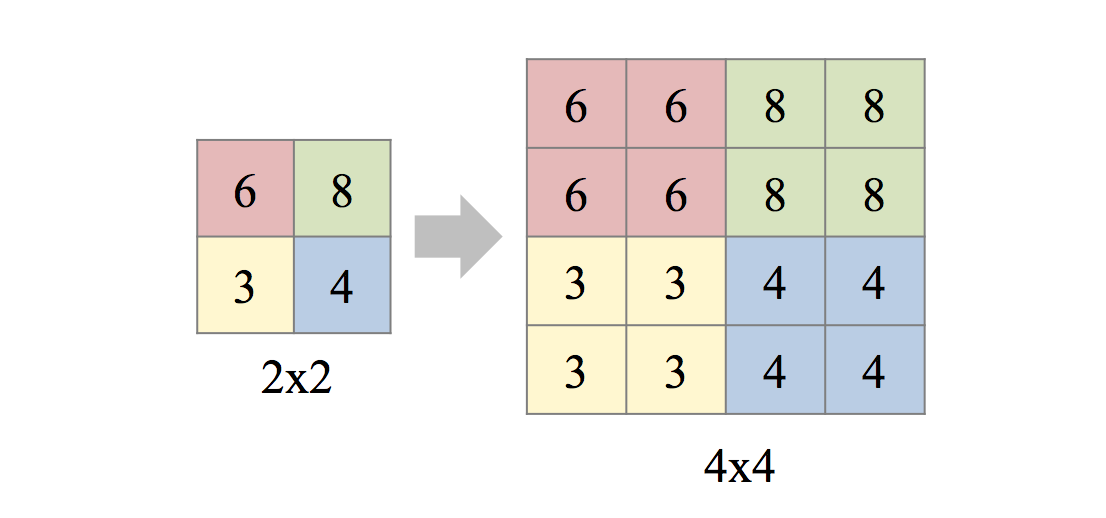
\includegraphics[width=.9\linewidth]{nnun.png}
\end{center}
\end{frame}


\begin{frame}{Max unpooling}
\begin{center}
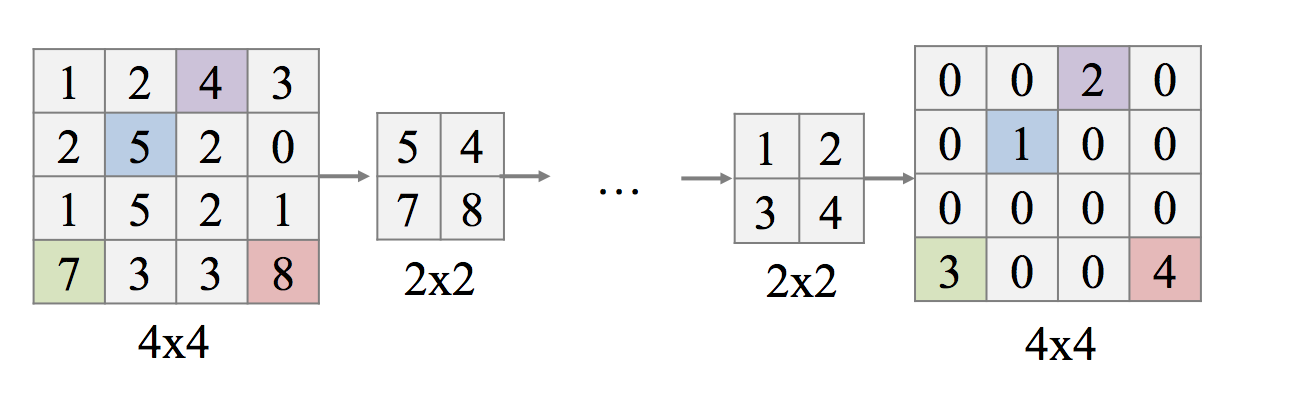
\includegraphics[width=.9\linewidth]{maxun.png}
\end{center}
\end{frame}


\begin{frame}{Learnable unpooling: Transpose convolution}
\begin{center}
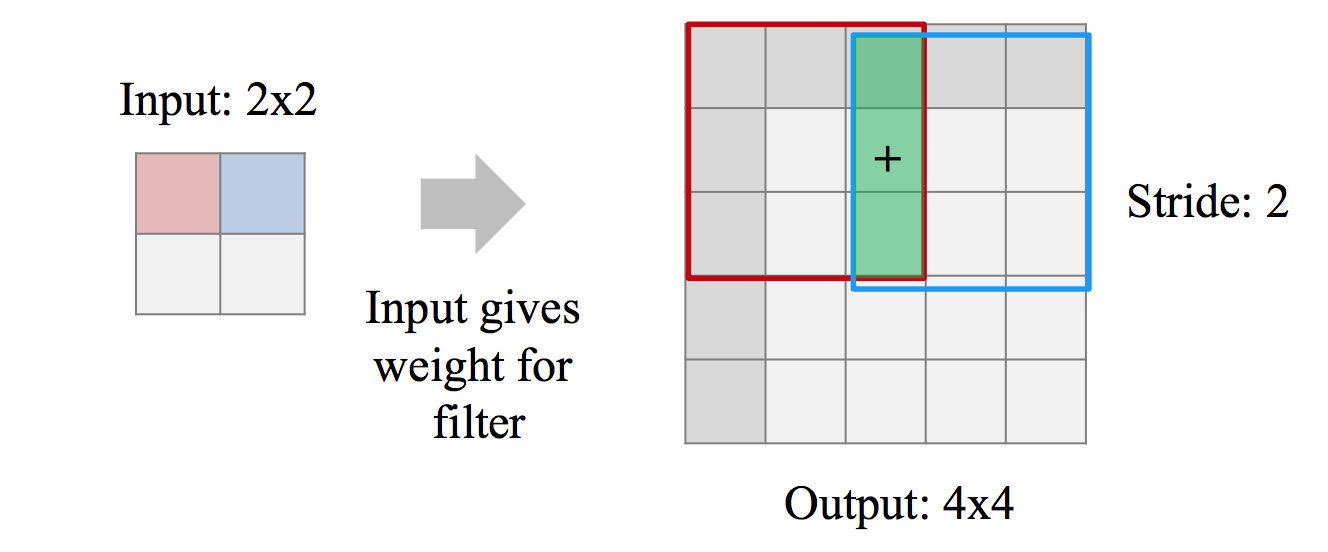
\includegraphics[width=.7\linewidth]{leun.png}
\end{center}
\begin{itemize}
	\item Каждую клетку надо распаковать в $4$ клетки $\Rightarrow$ свёртка $3 \times 3$ со сдвигом $2$
\end{itemize}
\end{frame}

\begin{frame}{Пример:}
\begin{center}
	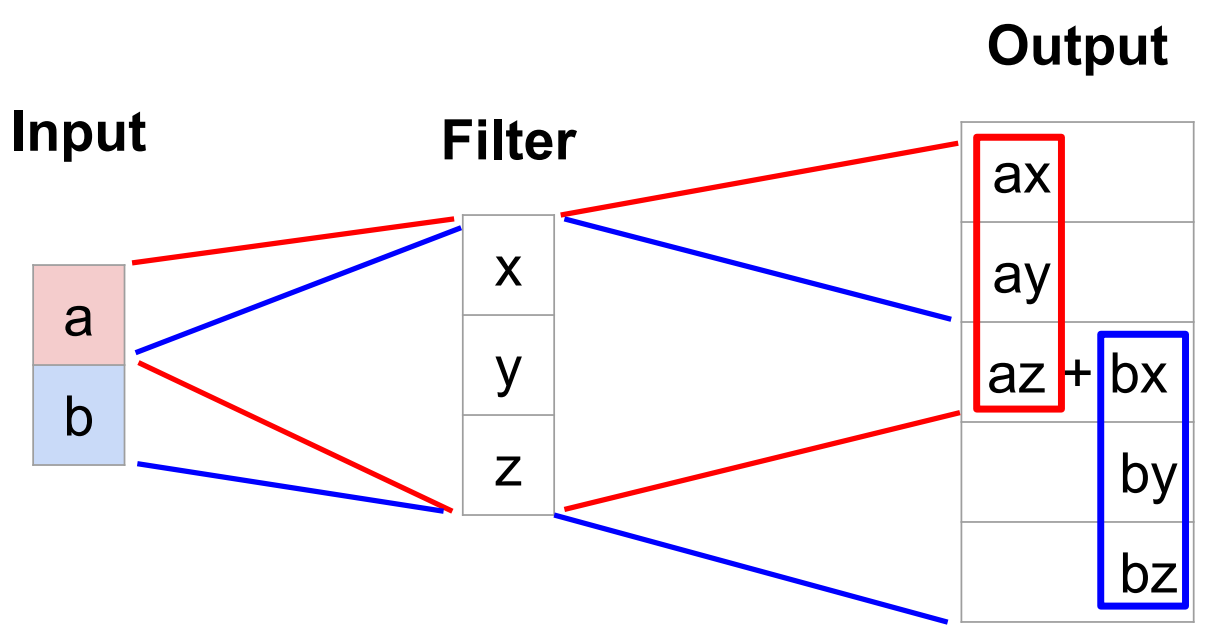
\includegraphics[width=.7\linewidth]{unpooling_example.png}
\end{center}
\end{frame}





\begin{frame}{Fully-convolution net}
\begin{center}
	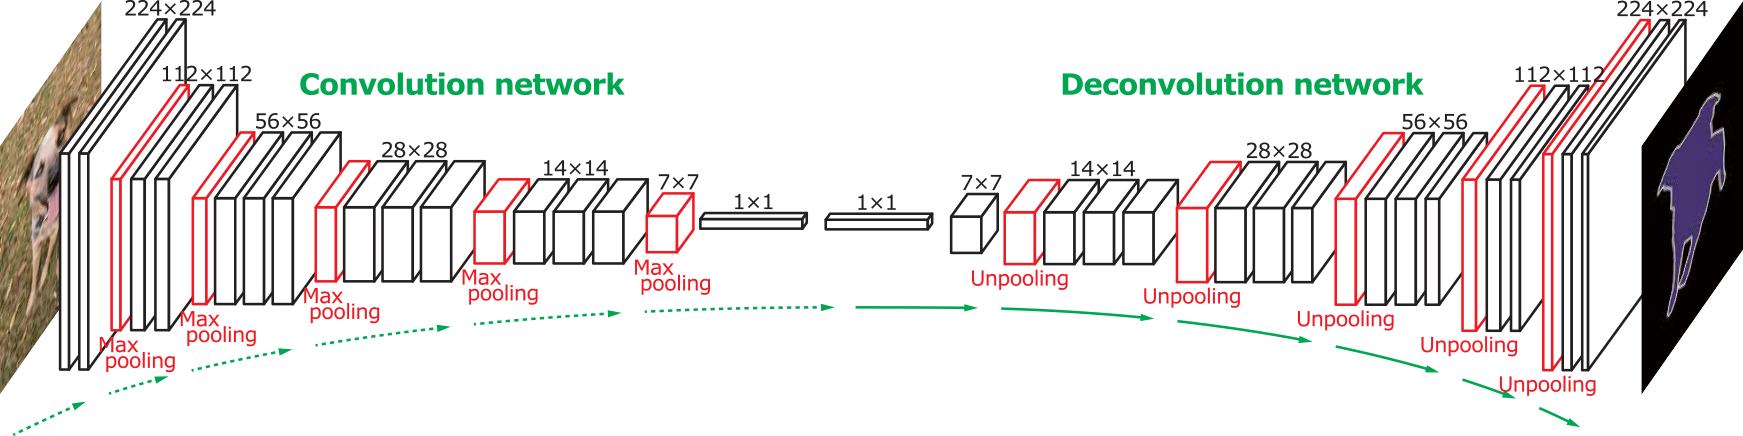
\includegraphics[width=.8\linewidth]{fully_net.png}
\end{center}
\begin{itemize}
	\item Cвернули в скрытое представление, развернули, спрогнозировали
\end{itemize}
\end{frame}


\begin{frame}{U-net}
\begin{center}
	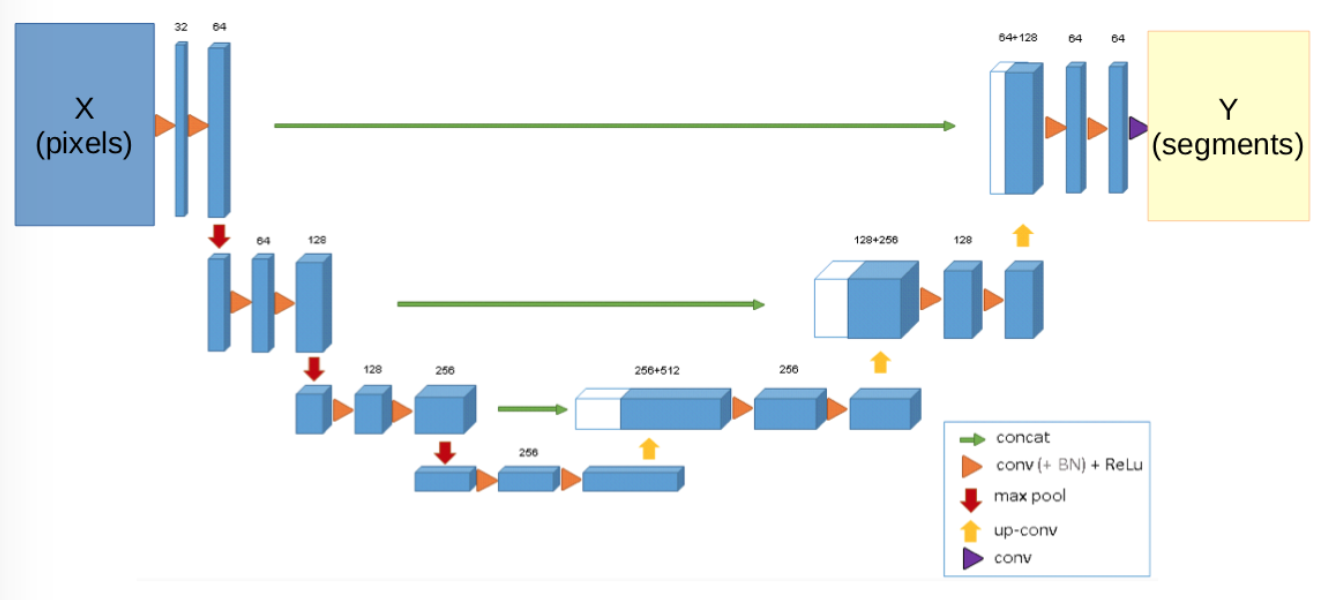
\includegraphics[width=.8\linewidth]{unet.png}
\end{center}
\begin{itemize}
	\item Можно добавить связи между слоями, отражающими одинаковую абстракцию, это должно улучшить модель
\end{itemize}
\end{frame}


 \begin{transitionframe}
	\begin{center}
		\Huge  Локализация изображения
	\end{center}
\end{transitionframe}

\begin{frame}{Примеры}
\begin{center}
	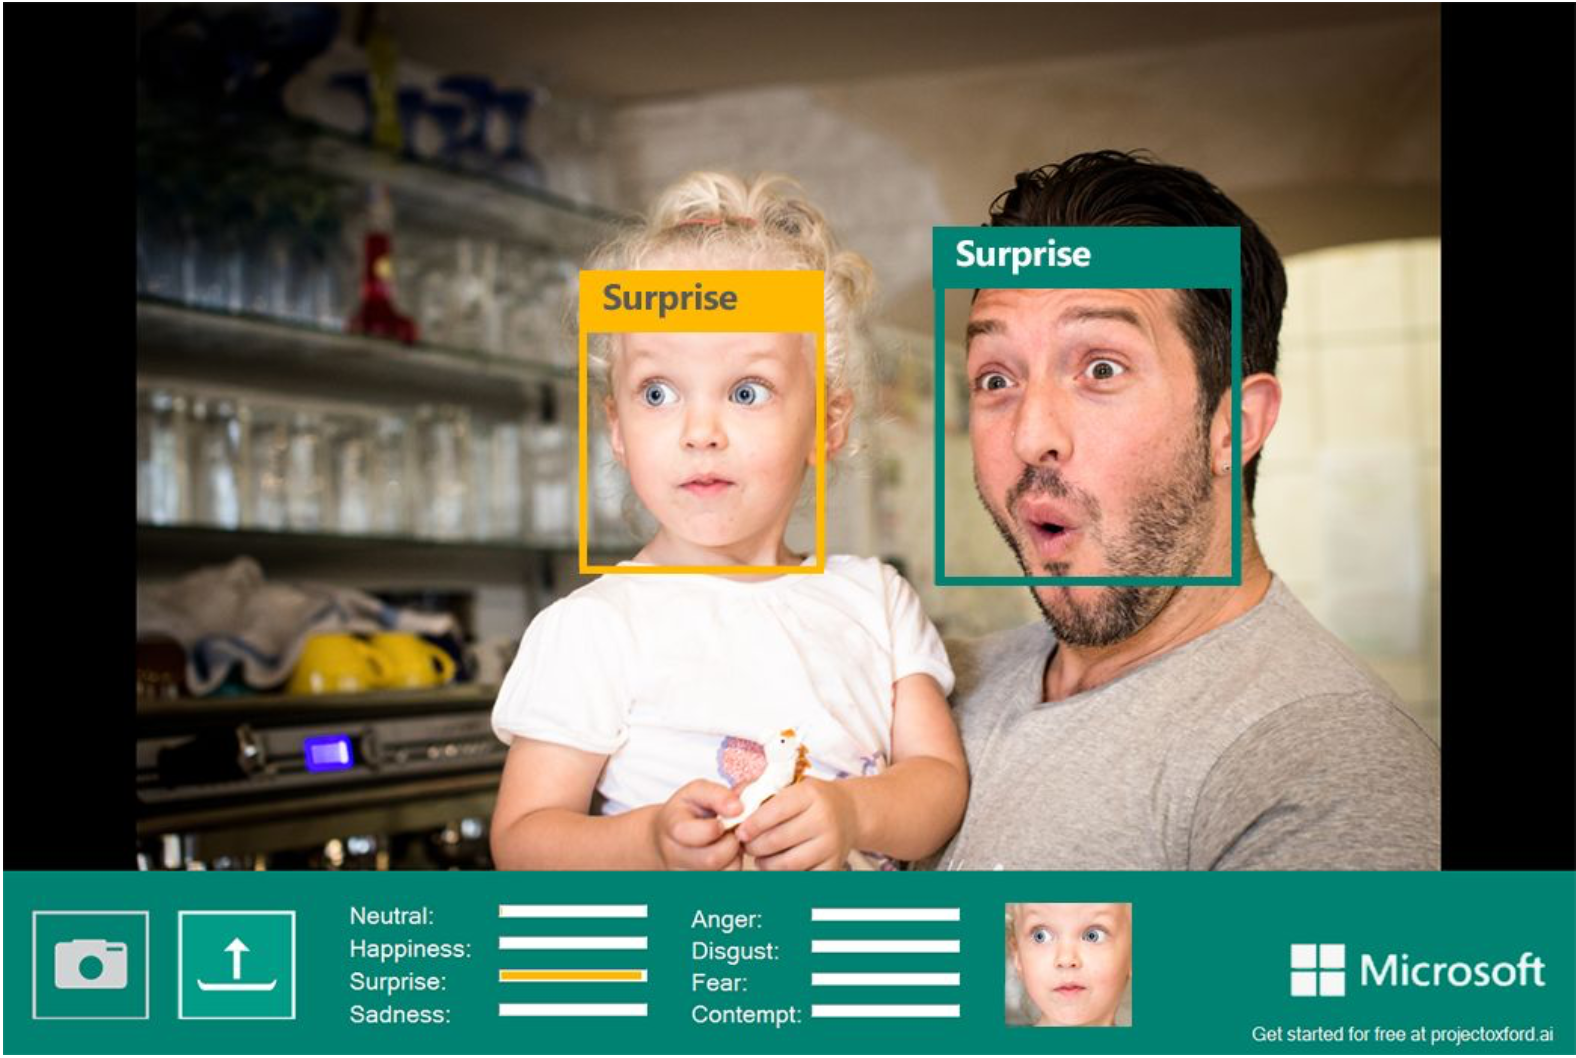
\includegraphics[width=.7\linewidth]{loc1.png}
\end{center}
\end{frame}


\begin{frame}{Примеры}
\begin{center}
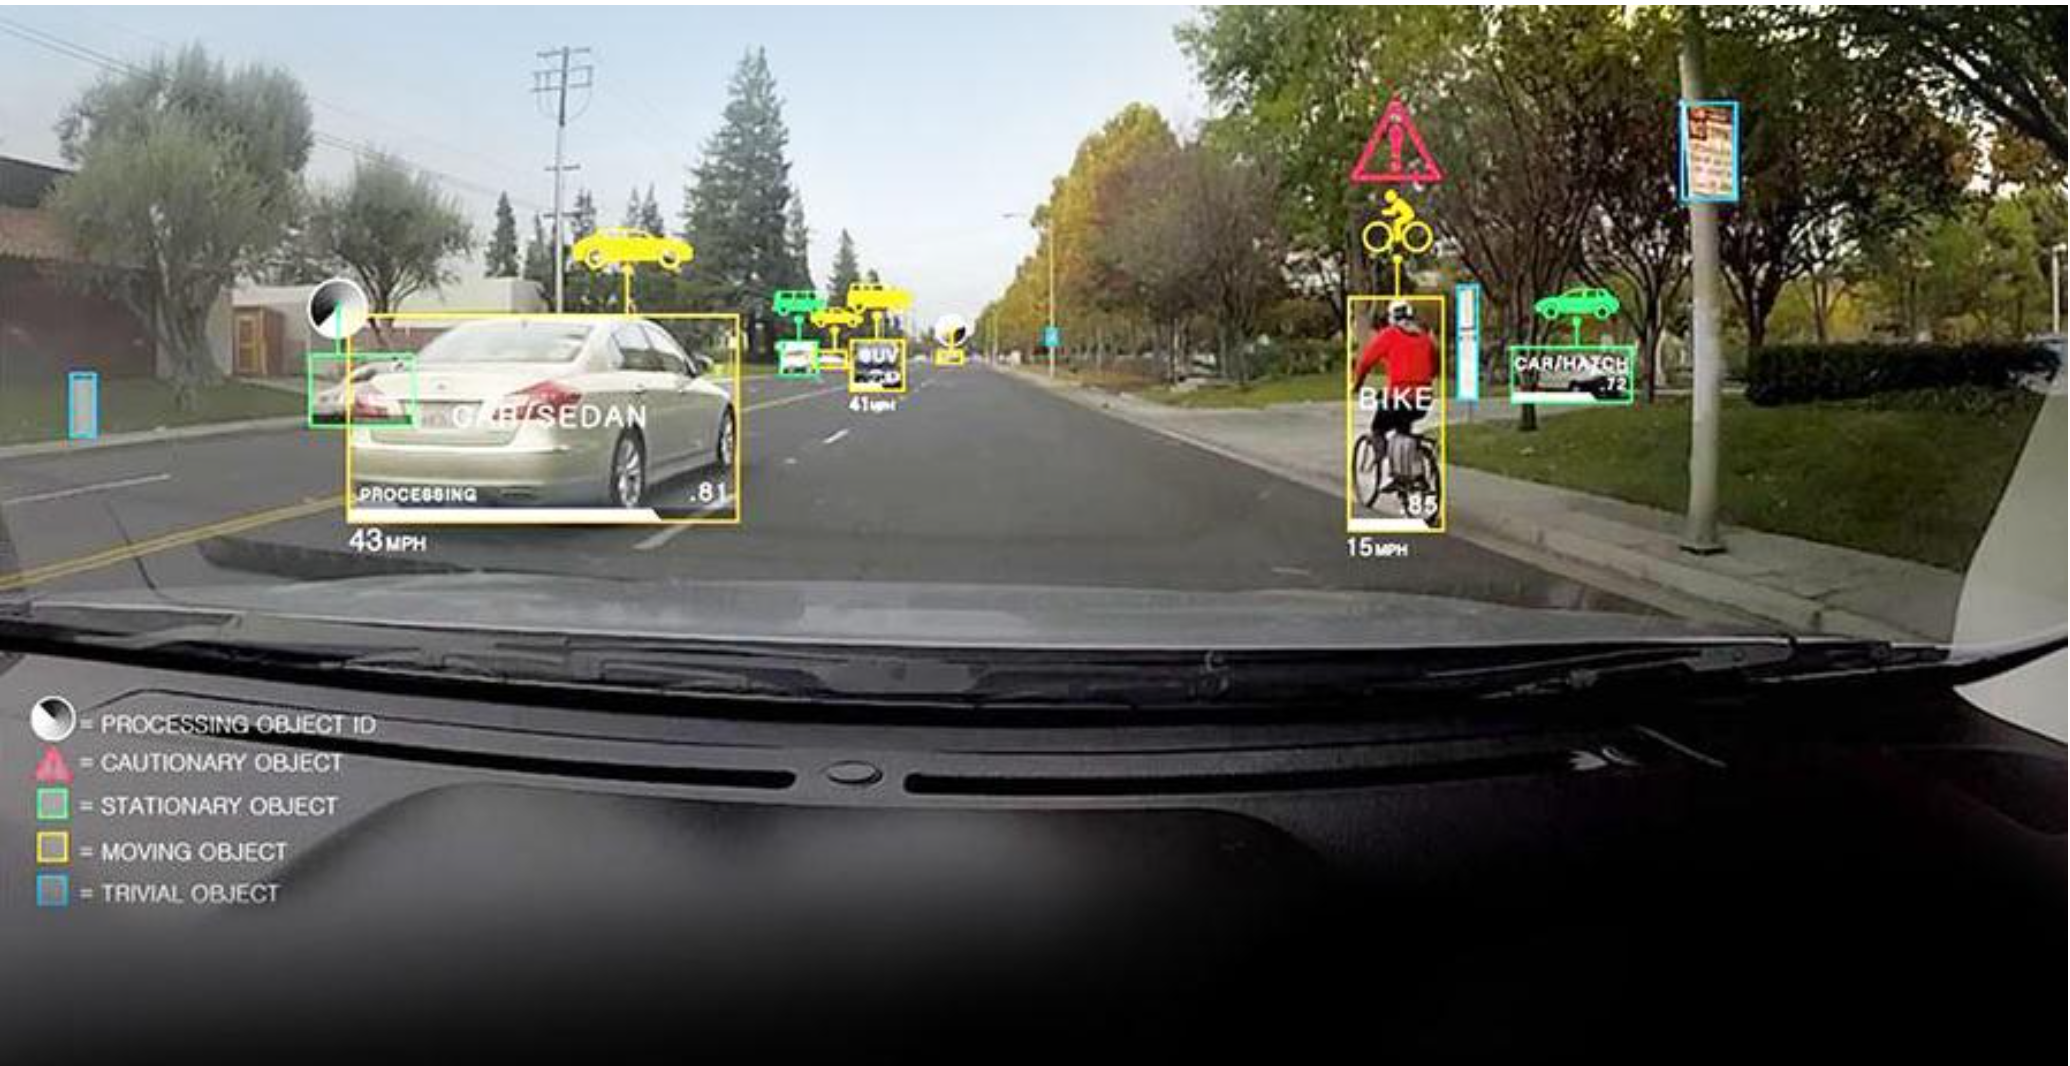
\includegraphics[width=.9\linewidth]{loc2.png}
\end{center}
\end{frame}

\begin{frame}{Локализация}
\begin{center}
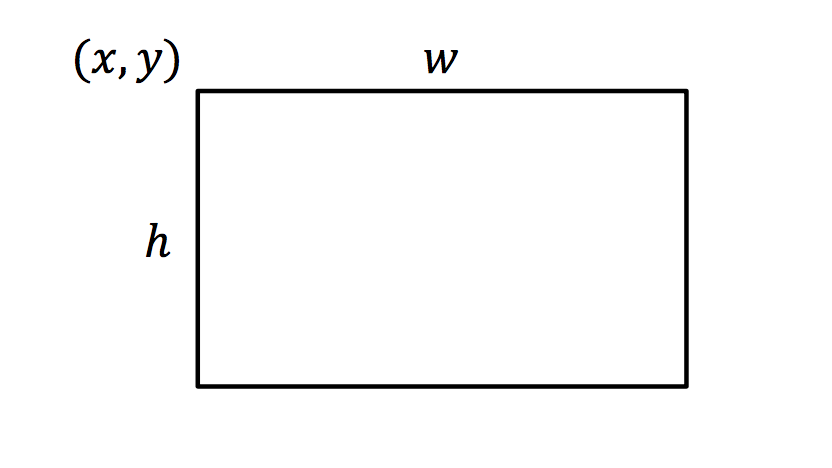
\includegraphics[width=.5\linewidth]{box.png}
\end{center}
\begin{wideitemize}
\item для локализации объекта нужно нащупать рамочку, в котором он находится
\item рамочка описывается параметрами $(x,y,w,h)$
\end{wideitemize}
\end{frame}

\begin{frame}{Локализация}
\begin{center}
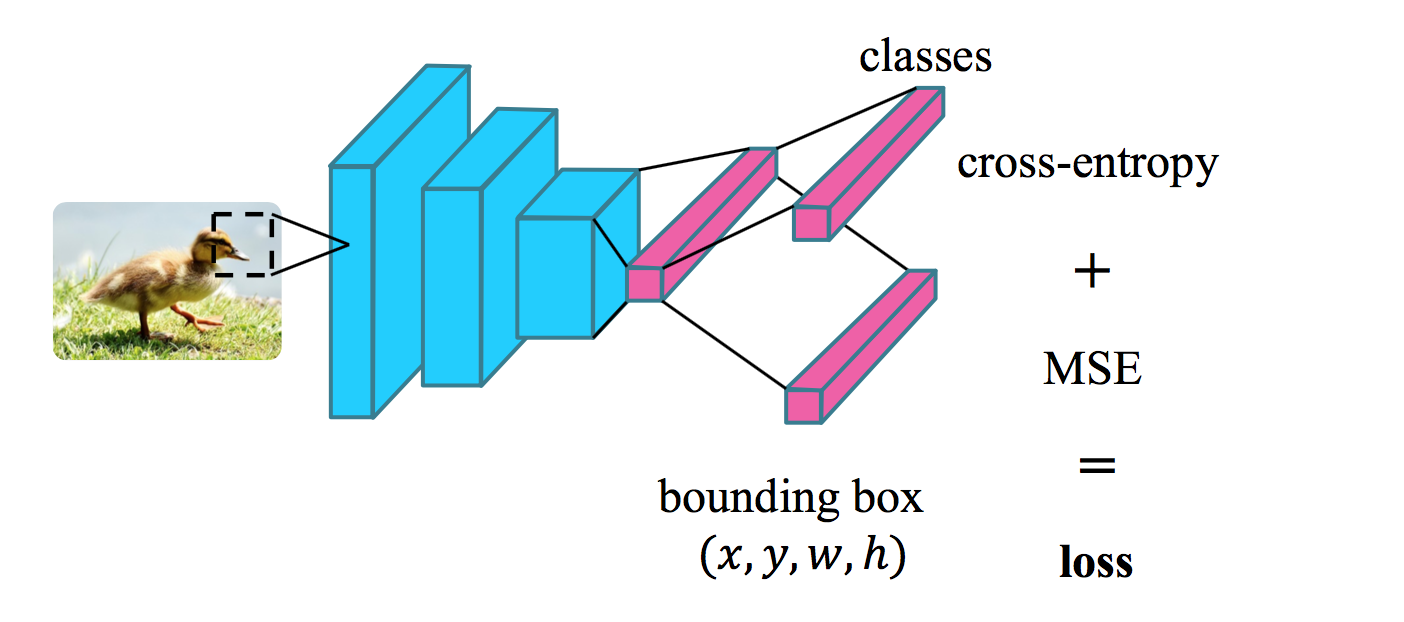
\includegraphics[width=.9\linewidth]{duck_3.png}
\end{center}
\end{frame}


\end{document}
